\documentclass[master=ecws,masteroption=ai,acyear=2019 -- 2020]{kulemt}
\setup{% Remove the "%" on the next line when using UTF-8 character encoding
  %inputenc=utf8,
  title={Reputation-driven Decision-making in Networks of Stochastic Agents},
  author={David Maoujoud},
  promotor={Prof.\,dr.\ L. De Raedt \and Dr.\ G. Rens},
  assessor={Prof.\,dr.\ M. Denecker\and Dr. \ F. Yang},
  assistant={Dr.\ G. Rens}}
% Remove the "%" on the next line for generating the cover page
%\setup{coverpageonly}
% Remove the "%" before the next "\setup" to generate only the first pages
% (e.g., if you are a Word user).
%\setup{frontpagesonly}

% Choose the main text font (e.g., Latin Modern)
\setup{font=lm}

% If you want to include other LaTeX packages, do it here. 

% Finally the hyperref package is used for pdf files.
% This can be commented out for printed versions.
%\usepackage[pdfusetitle,colorlinks,plainpages=false]{hyperref}
\usepackage[pdfusetitle,plainpages=false]{hyperref}

%%%%%%%
% The lipsum package is used to generate random text.
% You never need this in a real master's thesis text!
\IfFileExists{lipsum.sty}%
 {\usepackage{lipsum}\setlipsumdefault{11-13}}%
 {\newcommand{\lipsum}[1][11-13]{\par And some text: lipsum ##1.\par}}
%%%%%%%











%\usepackage{a4wide}
%\usepackage[a4paper]{geometry}
\usepackage[english]{babel}
\usepackage{graphicx}
\usepackage{url}

\newcommand{\RefVgl}[1]{~\textup{(\ref{#1})}} % using non breaking space, so use as\RefVgl{eq:foo}
\newcommand{\RefFig}[1]{Figure~\textup{\ref{#1}}}
\newcommand{\RefTab}[1]{Table~\textup{\ref{#1}}}
\newcommand{\RefSec}[1]{Section~\textup{\ref{#1}}}
\newcommand{\RefChap}[1]{Chapter~\textup{\ref{#1}}}
\newcommand{\RefThe}[1]{Theorem~\textup{\ref{#1}}}
\newcommand{\RefLem}[1]{Lemma~\textup{\ref{#1}}}
\newcommand{\RefGev}[1]{Corollary~\textup{\ref{#1}}}
\newcommand{\RefDef}[1]{Definition~\textup{\ref{#1}}}
\newcommand{\RefAlg}[1]{Algorithm~\textup{\ref{#1}}}

\newcommand{\RefEx}[1]{Example~\textup{\ref{#1}}}

\usepackage{amsmath,amsfonts,amsthm}
\usepackage{mathtools}

\bibliographystyle{vancouver}

\usepackage{subfig}


\usepackage{pgfplots}  
%\usepackage{SIunits} 
\pgfplotsset{compat=newest}




\usepackage{filecontents}
\usepackage{pgfplots, pgfplotstable}
\usepgfplotslibrary{statistics}

\usepackage{rotating,booktabs,multirow}

\usepackage{amssymb}


\usepackage{algorithm}
\usepackage[noend]{algpseudocode}

\makeatletter
\def\BState{\State\hskip-\ALG@thistlm}
\makeatother

\theoremstyle{plain}
  \newtheorem{theorem}{Theorem}[chapter]
  \newtheorem{lemma}[theorem]{Lemma}
  \newtheorem{corollary}[theorem]{Corollary}
\theoremstyle{plain}
  \newtheorem{definition}[theorem]{Definition}
  \newtheorem{example}[theorem]{Example}
\theoremstyle{remark}
  \newtheorem*{remark}{Remark}

\newcommand{\field}[1]{\mathbb{#1}} % the font for a mathematical field is blackboard
\newcommand{\R}{\field{R}} % the field of the reals
\newcommand{\N}{\field{N}} % the field of the natural numbers
\newcommand{\C}{\field{C}} % the field of complex number
\newcommand{\Z}{\field{Z}} % the field of integers
\newcommand{\E}{\field{E}}

\renewcommand{\vec}[1]{\boldsymbol{#1}} % vectors in bold instead of with an arrow on top
\newcommand{\convolution}{\ast} % convolution
\DeclareMathOperator{\diag}{diag}


\usepackage{xcolor}
\usepackage[intoc]{nomencl}  
\makenomenclature
\usepackage{xstring}
\usepackage{xstring}
\usepackage{xpatch}
\patchcmd{\thenomenclature}
  {\leftmargin\labelwidth}
  {\leftmargin\labelwidth\itemindent 1em }
  {}{}
\newcommand{\nomenclheader}[1]{
  \item[\hspace*{-\itemindent}\normalfont\bfseries#1]}
\renewcommand\nomgroup[1]{
  \IfStrEqCase{#1}{
   {A}{\nomenclheader{Acronyms}}
   {S}{\nomenclheader{Symbols}}
   {N}{\nomenclheader{Notation}}
  }
} 

\nomenclature[A]{MAS}{Multi-agent System}
\nomenclature[A]{MDP}{Markov Decision Process}
\nomenclature[A]{POMDP}{Partially Observable Markov Decision Process}
\nomenclature[A]{SARL}{Single-agent Reinforcement Learning}
\nomenclature[A]{SAL}{Single-agent Learning}
\nomenclature[A]{MARL}{Multi-agent Reinforcement Learning}
\nomenclature[A]{RL}{Reinforcement Learning}
\nomenclature[A]{VI}{Value iteration}
\nomenclature[A]{eVTOL}{Electric Vertical Take-off and Landing}
\nomenclature[A]{MAL}{Multi-agent Learning}

\nomenclature[N]{$e'$}{Value of $e$ at the following time-step}
\nomenclature[N]{$\mathcal{E}$}{Finite set of elements}
\nomenclature[N]{$\lvert \mathcal{E} \rvert$}{Cardinality of $\mathcal{E}$}

\nomenclature[N]{$\Delta (\mathcal{E})$}{Set of probability distributions over the elements of $\mathcal{E}$}


\nomenclature[N]{$\sum_{e}$}{Shorthand notation for $\sum_{e \in \mathcal{E}}$}

\nomenclature[N]{$\{X_g\}$}{Shorthand notation for $\{X_g \,\,\lvert\,\, g \in \mathcal{G}\}$}

\nomenclature[N]{$\mathcal{A} \oplus \mathcal{B}$}{Cross-sum of vectors $\mathcal{A}$ and $\mathcal{B}$, defined as $\{ a + b \,\,\lvert \,\, a \in \mathcal{A} \land b \in \mathcal{B} \}$}

\makeatletter
\newenvironment{chapquote}[2][2em]
  {\setlength{\@tempdima}{#1}%
   \def\chapquote@author{#2}%
   \parshape 1 \@tempdima \dimexpr\textwidth-2\@tempdima\relax%
   \itshape}
  {\par\normalfont\hfill--\ \chapquote@author\hspace*{\@tempdima}\par\bigskip}
\makeatother








%\includeonly{chap-n}
\begin{document}

\tableofcontents*

\begin{abstract}
This thesis studies multi-agent systems that involve networks of self-interested agents. In 2018, \textit{Rens et al.} \cite{rensetal} developed a Markov Decision Process-derived framework, called RepNet-POMDP, tailored to domains in which agent reputation is a key driver of the interactions between agents. The theoretical foundation of the framework was provided; the framework itself was, however, subsequently left unimplemented. 

\noindent Due to the highly intractable nature of its exact planning algorithm, we first reduce the framework to its fully observable equivalent, called RepNet-MDP, in an effort to study the framework's properties more efficiently. We further alleviate the intractability of the framework by devising an algorithm for finding approximate solutions. We show that the concept of \textit{directed actions}, as introduced by \textit{Rens et al.}, is subject to several theoretical inconsistencies, and propose an alternative interpretation of this concept that retains its core characteristics. We furthermore demonstrate that the initial notion of \textit{action distribution} can lead to undesirable agent behavior, and provide a revised formulation of the concept.

\noindent The viability of the framework is tested in a series of experiments designed to highlight its strengths and shortcomings. The tests display the RepNet agents' ability to leverage the framework's fundamental properties in an effort to adapt their behavior to the past behavior and reliability of the remaining agents of the network. RepNet agents are furthermore shown to be willing to sacrifice their selfish intentions in an attempt to maintain a general level of well-being of the entire network. Finally, our work identifies a limitation of the framework in its current formulation that prevents its agents from learning in circumstances in which they are not a primary actor.
\end{abstract}

% A list of figures and tables is optional
%\listoffigures
%\listoftables
% If you only have a few figures and tables you can use the following instead
\listoffiguresandtables
% The list of symbols is also optional.
% This list must be created manually, e.g., as follows:
\chapter{List of Abbreviations and Symbols}
\section*{Abbreviations}
\begin{flushleft}
  \renewcommand{\arraystretch}{1.1}
  \begin{tabularx}{\textwidth}{@{}p{12mm}X@{}}
    MAS   & Multi-agent System \\
    MDP   & Markov Decision Process \\
    POMDP  & Partially Observable Markov Decision Process \\
    SARL  & Single-agent Reinforcement Learning \\
    SAL  & Single-agent Learning \\
    MARL  & Multi-agent Reinforcement Learning \\
    MAL  & Multi-agent Learning \\
    RL  & Reinforcement Learning \\
    VI  & Value iteration \\
    eVTOL  & Electric Vertical Take-off and Landing \\
  \end{tabularx}
\end{flushleft}
\section*{Symbols}
\begin{flushleft}
  \renewcommand{\arraystretch}{1.1}
  \begin{tabularx}{\textwidth}{@{}p{12mm}X@{}}
    $e'$    & Value of $e$ at the following time-step \\
    $\mathcal{E}$   & Finite set of elements \\
    $\lvert \mathcal{E} \rvert$   & Cardinality of $\mathcal{E}$ \\
    $\Delta (\mathcal{E})$   & Set of probability distributions over the elements of $\mathcal{E}$ \\
    $\sum_{e}$ & Shorthand notation for $\sum_{e \in \mathcal{E}}$ \\
    $\{X_g\}$ & Shorthand notation for $\{X_g \,\,\lvert\,\, g \in \mathcal{G}\}$ \\
    $\mathcal{A} \oplus \mathcal{B}$ & Cross-sum of vectors $\mathcal{A}$ and $\mathcal{B}$, defined as $\{ a + b \,\,\lvert \,\, a \in \mathcal{A} \land b \in \mathcal{B} \}$ \\
    $\alpha$ & Learning rate\\
    $\gamma$ & Discount factor \\
    $\epsilon$ & Exploration-exploitation trade-off parameter \\
    $\eta$ & Laplace smoothing parameter\\
    $D$ & Look-ahead depth \\
    
  \end{tabularx}
\end{flushleft}









% Now comes the main text
\mainmatter



\chapter{Introduction}

%\begin{chapquote}{Louis Bloom, \textit{Nightcrawler}}
%``When it comes to your work reputation, you can’t unring the bell.''
%\end{chapquote}

\section{Context}



Markov Decision Processes (MDPs) form a mathematical framework for single-agent decision-making in stochastic environments \cite{Russell:2009:AIM:1671238}. They are characterized by the possible states of an environment of interest, the actions this environment is subject to, its dynamics, and a reward scheme. Solving an MDP yields a policy that instructs the agent on how to behave in each situation. One could, by way of illustration, use this formalism to provide an agent of interest, say, a robot to be deployed in a maze (i.e., the environment), with an optimal way of finding its way out (i.e., a policy). The robot changes the state of the environment by applying actions to it, that is, by moving about in the maze. In addition, one may describe the robot's movements as unreliable, thereby adding an element of stochasticity to the problem; the robot could, for instance, occasionally move further than anticipated. The interactions between the agent and the environment shape the dynamics of the problem.

Several extensions of the original framework have been proposed to accommodate for the presence of multiple agents. 
Some of them, most notably Multi-agent MDPs (MMDPs) \cite{Boutilier} and Decentralized Partially Observable MDPs (Dec-POMDPs) \cite{decmdp, decmdp2}, operate under the assumption that the agents are selfless and have a common goal. Others, such as Interactive-POMDPs (I-POMDPs) \cite{ipomdp}, make no such assumptions, and are designed for each agent to adapt its behavior to its self-centered peers'.


A primary concern when dealing with self-centered agents is that it makes multi-agent learning inherently more complex than single-agent learning \cite{nonstation, convergence}. This is, to a large extent, due to the fact that each agent needs to take into account the behavior of the entire network of agents when learning its own behavior. Additionally, agent behavior tends to be ever-changing. This \textit{non-stationarity} of agent behavior leads to the loss of policy \textit{convergence} properties that can often be found in single-agent formalisms \cite{convergence}. 


The paper "\textit{Maximizing Expected Impact in an Agent Reputation Network}" published in 2018 by Rens et al. \cite{rensetal} proposes a mathematical framework called \textit{RepNet-POMDP} designed to handle domains in which an agent's reputation among other agents dictates its behavior. The framework builds on top of the MDP framework, by explicitly modeling agent behavior and reputation, as well as introducing partial observability of the environment and other agents' behavior. 

Understanding decision-making in the face of selfishness plays an important role in several domains and is notably the subject of \textit{game theory} \cite{repp}. A simple trading scenario can serve as an illustrative example. Let two agents constitute the two parties involved in a trade transaction. The first agent, called the buyer, wishes to buy a good offered by the second agent, called the seller. The seller is at no point forced to accept the trade offer: in fact, if the buyer is known to have a poor reputation, the seller might prefer to refuse the trade offer to steer clear of any interactions with the buyer. The reputation of the buyer shapes the dynamics of the interactions between both agents.

A second and more complex example in which an agent's reputation plays a key role revolves around the topic of Electric Vertical Take-off and Landing aircraft \cite{vtol}. In this illustrative example, these pilotless aircraft make up a network of agents that require air traffic management.
The example furthermore involves a set of vertiports that the aircraft can land on to recharge their batteries. The aircraft are to carry passengers from one vertiport to another. Say a first air-taxi is currently charging its battery while a second one is in the air waiting for the vertiport to free up. As the second aircraft's battery reaches lower levels, it must either fly to another nearby vertiport or trust the first aircraft to leave. This decision is to be made based on the first aircraft's past behavior and reputation.

The RepNet framework is tailored to problems alike and constitutes the subject of the present thesis. In their paper, \textit{Rens et al.} provide the theoretical foundation of the framework, which introduces several concepts that distinguish it from other MDP-derived frameworks. As such, the notions of \textit{action distribution}, \textit{image}, \textit{reputation}, and \textit{directed actions} are established as key components of the framework, and are used by RepNet agents to navigate through the environment and interact with the other agents that are apart of the environment. While these concepts were developed on a theoretical level, the framework itself was not evaluated empirically.

\paragraph{Problem statement:} \textit{The primary goal of the present thesis is to study the properties of the RepNet framework, and evaluate its viability as an MDP-derived, multi-agent framework that deals with agent selfishness. Finding exact solutions for RepNet-POMDPs is, however, known to be computationally \textit{intractable}. The intractability of the framework is to be alleviated before the framework and its properties can be tested.}

\paragraph*{}The study of the framework's properties can be further refined into four research questions, which will be answered in this thesis.

\paragraph{Research question 1:} \textit{Are the concepts of action distribution, image, and reputation effective in practice?}

\paragraph{Research question 2:} \textit{Is the concept of directed actions effective in practice?}

\paragraph{Research question 3:} \textit{Are RepNet agents capable of drawing general conclusions on the interactions between the agents that are apart of the environment?}

\paragraph{Research question 4:} \textit{Are RepNet agents capable of being cooperative in spite of their selfish intentions?}






\paragraph*{}Broadly speaking, the work carried out in regards to the RepNet framework involves a first part of \textit{theoretical}, and a second part of \textit{experimental}, nature.

\paragraph*{\textit{Theoretical part:}} The approach taken in this thesis to alleviate the problem of intractability can be summarized as a two-step procedure: the first step consists in reducing the framework to a fully observable setting called RepNet-MDP. The second step consists in favoring approximate solutions to the reduced framework of satisfactory quality over exact solutions. An algorithm for finding approximate solutions will be presented to this end.

\paragraph*{\textit{Experimental part:}} After reducing the framework's intractability, the viability of said framework will be evaluated in a series of simplified scenarios drawn from the \textit{trading} and \textit{air-taxi} domains. Each scenario will be tailored to showcase the strengths and shortcomings of the framework.



\section{Outline}
This thesis is structured in the following way: \RefChap{chap:background} summarizes the relevant background required. \RefChap{chap:related} provides an overview of the related work and, in particular, the framework proposed by \textit{Rens et al.} \cite{rensetal}. \RefChap{chap:mdp} then discusses the reduction of the starting framework to a fully observable setting. The experimental setup of the reduced framework is given in \RefChap{chap:method}. \RefChap{chap:res} provides the experimental results and discusses the strengths and shortcomings of the RepNet framework. Finally, the work of the previous chapters is brought together and summarized in \RefChap{chap:conclusion}.


\chapter{Background}
\label{chap:background}
The present chapter covers background information referred to throughout the thesis. A brief introduction to the \textit{Reinforcement Learning Problem} is first given in \RefSec{sec:rl}. Two Single-agent Markov Decision Process frameworks are then introduced in \RefSec{sec:sarl}. The time complexity of exact solutions to these problems is analyzed in \RefSec{sec:intract}. An overview of several exact and approximate solving techniques is given in \RefSec{sec:stateart}. Finally, \RefSec{sec:repstat} briefly discusses \textit{first-order} representations of Markov Decision Processes.
\section{The Reinforcement Learning Problem}
\label{sec:rl}
Reinforcement Learning (RL) is a Machine Learning paradigm, in which a learning entity, typically called agent, learns in an environment by performing actions and observing the environment's response \cite{RLgeneral}. More specifically, when an agent performs action $a_t$ at time $t$, the environment, initially in state $s_t$, returns its new state $s_{t+1}$ as well as a reward $r_{t+1}$ to the agent. The agent aims to maximize the reward it can accumulate over time. The general feedback loop is schematized in \RefFig{fig:feedback}.

\begin{figure}[h]
  \begin{center}
    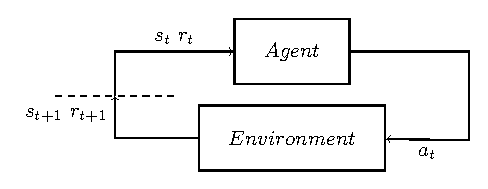
\includegraphics{images/MasterThesisRLLoop.pdf}
  \end{center}
  \caption{Reinforcement Learning feedback loop}\label{fig:feedback}
\end{figure}

The RL paradigm can be formalized in Single-agent and Multi-agent settings. Several properties emerging from the former no longer hold in the latter. The fundamental single-agent formalisms are now covered in further detail.

\section{Single-agent formalisms}
\label{sec:sarl}
This section formalizes the fundamental concepts of learning in single-agent settings. In the present thesis, the following properties of the environment are assumed to be true:
\begin{itemize}
    \item The environment behaves stochastically, meaning that given a starting state and an action performed, the environment is not guaranteed to transition to the same new state each time. A robot expected to jump forward one meter might, for instance, miss the target and jump too far.
    \item The environment is stationary, meaning that the transition rules which the environment abides by do not change over time. 
    \item The environment obeys the \textit{Markov property}. This property states that the probability of the environment transitioning to any given state is solely conditioned by the current state of the environment and the current action of the agent \cite{Russell:2009:AIM:1671238}.
    \item The state space is discrete and comprised of a finite number of elements. 
\end{itemize}
\RefSec{sec:mdp} covers the simplest form of Markov Decision Processes. \RefSec{sec:pomdp} then introduces a common extension to the initial framework.

\subsection{Fully Observable Markov Decision Processes}
\label{sec:mdp}
The Single-Agent Learning (SAL) problem can be formally modeled as a Markov Decision Process.
\begin{definition}[Fully Observable MDP]
\label{def:fomdp}
A fully observable Markov Decision Process, or simply MDP, $\mathcal{M}$ is formally defined as a tuple \cite{Russell:2009:AIM:1671238}
\begin{align*}
    \mathcal{M} := \big \langle \mathcal{S}, \mathcal{A}, \mathcal{T}, \mathcal{R} \big \rangle
  \end{align*}
where:
\begin{itemize}
    \item $\mathcal{S}$ is the set of possible states of the environment.
    \item $\mathcal{A}$ is the set of possible actions.
    \item $\mathcal{T} : \mathcal{S} \times \mathcal{A} \times \mathcal{S} \rightarrow [0,1]$ is called the \textit{transition model}. $\mathcal{T}(s,a,s')$ returns the probability of the environment transitioning from state $s$ to state $s'$ after action $a$ is performed.
    \item $\mathcal{R}: \mathcal{S} \times \mathcal{A} \rightarrow \R$ is called the \textit{reward function}. $\mathcal{R}(s,a)$ returns the immediate reward received after performing action $a$ in state $s$.
\end{itemize}
\end{definition}
The objective of an MDP agent is to maximize its long-term cumulative reward, called \textit{utility}. While the utility can be defined in several ways, the most commonly used definition is called \textit{discounted future reward}. The utility $U$ of a \textit{finite} state-action sequence, sometimes called \textit{episode}, $E = \big \langle s_0,a_0,s_1, a_1,..., s_T, a_T \big \rangle$ is defined as \cite{Nitti2017}:
\begin{align}
\label{eq:utility}
    U(E) = \sum_{t=0}^{T} \gamma^t \mathcal{R}(s_t, a_t)
\end{align}
where $\gamma \in [0,1]$ is called the \textit{discount factor}. An agent moves about in the environment by following a \textit{policy}.

\begin{definition}[Finite-horizon policy]
\label{def:policymdp}
A finite-horizon policy $\pi : \mathcal{S} \times \N \rightarrow \mathcal{A}$ is a function that maps each environment state and remaining time-steps to the action the agent should take.
\end{definition}
The \textit{expected utility}, or \textit{value}, of being in any state $s_t$ at time-step $t$, while following policy $\pi$, with $d$ time-steps remaining, is defined as \cite{Nitti2017}:
\begin{align}
    V^{\pi}(s_t, d) = \E[U(E_t) \, | \, s_t, \pi] = \E \big[ \sum_{k = t }^{t+d} \gamma^{k-t} \mathcal{R}(s_k, a_k) \, \big| \, s_t, \pi \big ]
\end{align}
where $E_t$ is the sub-sequence of $E$ starting at time-step $t$. An optimal policy $\pi^\star$ is a policy such that
\begin{align}
    \forall s \in \mathcal{S}, \forall d \in \N, \forall \pi : V^{\star}(s,d) \geq V^{\pi}(s,d) 
\end{align}
where $V^{\star} : \mathcal{S} \times \N \rightarrow \R$ is the value function associated with optimal policy $\pi^{\star}$.
This policy satisfies the \textit{optimality equations}, also known as the \textit{Bellman equations}:
\begin{align}
\label{eq:bellman}
        \begin{dcases}
            V^{\star}(s, d) := \max_{a \in \mathcal{A}} \Big\{ \mathcal{R}(s,a) + \gamma \sum_{s' \in \mathcal{S}} \mathcal{T}(s,a,s') V^{\star}(s', d-1) \Big\}  &\forall s \in \mathcal{S}, d > 1
            \\
            V^{\star}(s, 1) := \max_{a \in \mathcal{A}} \Big\{ \mathcal{R}(s,a) \Big\} &\forall s \in \mathcal{S}
        \end{dcases}
    \end{align}
    
MDPs are adequate for modeling a range of stochastic domains in which the state of the environment is fully observable at all times. Yet, fully observable environments can not always be taken for granted. The problem of partial observability is covered hereafter.

\subsection{Partially Observable Markov Decision Processes}
\label{sec:pomdp}
Alongside the stochastic nature of many environments, a prevalent form of uncertainty lies in the partial observability of several domains. Take a robot equipped with proximity sensors advancing in a room filled with obstacles. This robot does not sense the actual state of the room. Rather, it can only sense what the sensors pick up, and may very well bump into obstacles that were missed during the sensing process. Partially Observable Markov Decision Processes are an extension of classic MDPs that deal with the problem of partial observability \cite{Russell:2009:AIM:1671238}.
\begin{definition}[Partially Observable MDP]
A partially observable MDP, or POMDP, $\mathcal{P}$ is formally defined as a tuple
\begin{align*}
    \mathcal{P} := \big \langle \mathcal{S}, \mathcal{A}, \mathcal{T}, \mathcal{R}, \Omega, \mathcal{O} \big \rangle
  \end{align*}
where:
\begin{itemize}
    \item $\mathcal{S}$, $\mathcal{A}$, $\mathcal{T}$ and $\mathcal{R}$ are defined as in \RefDef{def:fomdp}.
    \item $\Omega$ is the set of observations.
    \item $\mathcal{O} : \mathcal{A} \times \mathcal{S} \times \Omega \rightarrow [0,1]$ is called the \textit{observation function} or \textit{sensor model}. $\mathcal{O}(a,s',o)$ returns the probability of making observation $o$ after performing action $a$ and the environment transitioning to state $s'$.
\end{itemize}
\end{definition}
Instead of working with the actual states of the environment, the POMDP framework introduces the notion of \textit{belief states}.
\begin{definition}[Belief state]
A belief state $b \in \Delta(\mathcal{S})$ is a probability distribution over the possible states of the environment. As such, $b(s)$ returns the probability of being in state $s$. Furthermore,
\begin{align*}
    \sum_{s \in \mathcal{S}} b(s) = 1
\end{align*}
\end{definition}
Suppose the agent makes observation $o$ after taking action $a$ in current belief state $b$. The updated belief state $b'$ is computed using the \textit{state estimation function} $SE$ defined as follows:
\begin{align}
\label{eq:belief}
    b' := SE(b,a,o) := \Big\{(s',p) \,\,\Big| \,\,s' \in \mathcal{S} \land p =  \frac{\mathcal{O}(a,s',o) \sum_{s} \mathcal{T}(s,a,s') b(s)}
    {P(o | b, a)} \Big\}
\end{align}
where $P(o | b,a) = \sum_{s' \in \mathcal{S}} \mathcal{O}(a,s',o) \sum_{s \in \mathcal{S}} \mathcal{T}(s,a,s') b(s)$ is a normalizing constant.
The optimal value function $V^{\star} : \Delta(\mathcal{S}) \times \N \rightarrow \R$ satisfies the following \textit{optimality equations} (\forall b \in \Delta(\mathcal{S})):

\begin{align}
        \begin{dcases}
            V^{\star}(b, d) := \max_{a \in \mathcal{A}} \Big\{ \sum_{s \in \mathcal{S}}\mathcal{R}(s,a) b(s) + \gamma \sum_{o \in \Omega} P(o | b,a) V^{\star}(SE(b,a,o), d-1) \Big\}  
            \\
            V^{\star}(b, 1) := \max_{a \in \mathcal{A}} \Big\{ \sum_{s \in \mathcal{S}}\mathcal{R}(s,a) b(s) \Big\} 
        \end{dcases}
    \end{align}


\section{Time complexity of solving Markov Decision Processes via Value Iteration}
\label{sec:intract}
The present section covers the time complexity of a solving strategy for fully and partially observable MDPs called the value iteration algorithm. Partial observability is shown to render the computation of exact solutions intractable, even in single-agent settings.

Value iteration (VI) is an iterative process that considers successively longer planning horizons to produce exact, i.e. optimal, solutions to fully and partially observable MDPs \cite{phdthesispomdp}. This is accomplished by computing the $i$-th horizon optimal value function at each iteration $i$, using the $i-1$-th horizon optimal value function computed at the previous iteration. The termination criterion is different for infinite- and finite-horizon problems: in infinite horizon problems, termination is reached when the value function converges, i.e., when it no longer changes sufficiently between two iterations. The final value function is then kept. In finite-horizon problems, termination is reached when the value function has been computed for each step within the horizon depth. The value functions produced at each step are all kept. The fully observable MDP VI algorithm was introduced by \textit{Bellman} in 1957 \cite{Bellman:1957}, while \textit{Sondik} developed its counterpart for partially observable environments in the early 1970s \cite{sondik1973}.
\subsection{VI for fully observable, finite-horizon MDPs}
Let $\mathcal{M}$ be a finite horizon MDP of horizon $d$, $|\mathcal{S}|$ the number of states, and $|\mathcal{A}|$ the number of actions of $\mathcal{M}$. Each iteration $i$ of the VI planning algorithm computes the optimal value $V^{\star}(s,i)$ for each state $s$, i.e. $|\mathcal{S}|$ computations in total. Each such computation involves the maximization over $|\mathcal{A}|$ actions. For each action $a$, the evaluation involves the summation over $|\mathcal{S}|$ states. The time complexity of the VI algorithm is thus \cite{mdpcomp}
\begin{align}
    \mathcal{O}(d |\mathcal{S}|^2|\mathcal{A}|).
\end{align}
The algorithm is given in \RefAlg{alg:valitmdp}.

\begin{algorithm}[H]
\caption{Value iteration for finite-horizon MDPs}\label{alg:valitmdp}
\begin{algorithmic}[1]
\Procedure{Value-Iteration}{}
    
\For {$i = 1 \rightarrow d$}
    \ForAll{$s \in \mathcal{S}$} 
        \If {$i == 1$} \State $V^{\star}(s, 1) \leftarrow \max_{a \in \mathcal{A}} \Big\{ \mathcal{R}(s,a) \Big\}$
         \Else \State $V^{\star}(s, i) \leftarrow \max_{a \in A} \Big\{ \mathcal{R}(s,a) + \gamma \sum_{s' \in S} \mathcal{T}(s,a,s') V^{\star}(s', i-1) \Big\}$
        \EndIf
    \EndFor
\EndFor

\EndProcedure
\end{algorithmic}
\end{algorithm}
As such, MDP VI is polynomial in the number of states $|\mathcal{S}|$. The algorithm is said to be \textit{tractable} and belongs to complexity-class \textbf{P}.
\subsection{VI for partially observable, finite-horizon MDPs}
VI is less straightforward with POMDPs than with fully observable MDPs. This comes as a direct result of the belief space being continuous, making it impossible to compute $V^{\star}(b,n)$ for each belief state $b$ the way it is done for fully observable MDPs \cite{Russell:2009:AIM:1671238}. \\ The optimal value function $V^{\star}$ turns out to always be \textit{piecewise linear} and \textit{convex} in the belief space \cite{RePEc:inm:oropre:v:21:y:1973:i:5:p:1071-1088}. Formally, this equates to $V^{\star}$ having the following form:
\begin{align}
    V^{\star}(b, n) = \max_{\alpha \in \mathcal{V}_n} \sum_{s \in \mathcal{S}}\alpha(s) b(s) = \max_{\alpha \in \mathcal{V}_n} \alpha \cdot b
\end{align}
where $\mathcal{V}_n = \{\alpha_0,\alpha_1,...,\alpha_m \}$ is a set of $\alpha$-vectors, each $\alpha$-vector maintaining the parameters of an $|\mathcal{S}|$-dimensional hyperplane describing the optimal value function over a region of the belief space \cite{Pineau-2003-8730}. In other words, $V^{\star}$ is the upper surface of the collection of hyperplanes described by the $\alpha$-vectors \cite{uppersurface}. Each $\alpha$-vector is associated with a specific conditional plan, that is, the region over which one hyperplane in $\mathcal{V}_n$ dominates all other hyperplanes in $\mathcal{V}_n$ is associated with one optimal action. Each iteration $i$ of the algorithm  consists of two steps \cite{phdthesispomdp}:
\begin{itemize}
    \item Generation of potentially useful $i$-th horizon $\alpha$-vectors. This step first consists of the generation of $\mathcal{O}(|A||\Omega||\mathcal{V}_{i-1}|)$  projections in total. The algorithm then proceeds to compute $\mathcal{O}(|A||\mathcal{V}_{i-1}|^{|\Omega|})$ cross-sums. Each $\alpha$-vector is computed in $\mathcal{O}(|S|^2)$ time \cite{Pineau-2003-8730,hauskrecht,crosssum}. The generation step thus has a worst-case complexity 
    \begin{align}
        \mathcal{O}(|S|^2|A||\mathcal{V}_{i-1}|^{|\Omega|})
    \end{align}
    \item Pruning of fully-dominated $\alpha$-vectors. This step usually involves the solving of a linear program and does not add to the asymptotic complexity of the algorithm \cite{KAELBLING199899}.
\end{itemize}
The corresponding algorithm is given in \RefAlg{alg:valitpo}. Solving POMDP via VI is exponential in $|\Omega|$ and, as such, is said to be \textit{intractable}. While the notion of \textit{intractability} will be formalized in \RefChap{chap:related}, it is worth noting at this point that the \textit{intractability} of this single-agent-based algorithm is evocative of the challenges encountered in most multi-agent learning settings.

\begin{algorithm}[H]
\caption{Value iteration for finite-horizon POMDPs}\label{alg:valitpo}
\begin{algorithmic}[1]
\Procedure{Value-Iteration}{}


\ForAll{$a \in \mathcal{A}$} 
    \State $\mathcal{V}_1^{-} \leftarrow \alpha^{a,*}(s) = {R}(s,a)$
\EndFor
    
\For {$i = 2 \rightarrow d$}
    \ForAll{$a \in \mathcal{A}$} 
        \State $\mathcal{V}_i^{a,*} \leftarrow \alpha^{a,*}(s) = \mathcal{R}(s,a)$
            \ForAll{$o \in \Omega$} 
                \ForAll{$\alpha_{j} \in \mathcal{V}_{i-1}^{-}$} 
                    \State $\mathcal{V}_i^{a,o} \leftarrow \alpha_j^{a,o}(s) = \gamma \sum_{s' \in \mathcal{S}} \mathcal{T}(s,a,s') \mathcal{O}(a,s',o) \alpha_{j}(s')$
                \EndFor
            \EndFor
        \EndFor
        \ForAll{$a \in \mathcal{A}$}
            \State $\mathcal{V}_i^{a} = \mathcal{V}_i^{a,*} \oplus \mathcal{V}_i^{a,o_1} \oplus ... \oplus \mathcal{V}_i^{a,o_{|\Omega|}}$
        \EndFor
        \State $\mathcal{V}_i = \bigcup_{a \in \mathcal{A}} \mathcal{V}_i^a$
        \State $\mathcal{V}_i^{-} = \text{PRUNE}(\mathcal{V}_i)$
    \EndFor
\EndProcedure
\end{algorithmic}
\end{algorithm}
%As such, in accordance with equation (\ref{eq:intract}), POMDP VI is \textit{intractible}, regardless of the pruning strategy used \cite{intractt}.
\section{Model-based solving techniques}
\label{sec:stateart}
Various algorithms have followed since the introduction of VI. The present section first provides an overview of the different algorithm classes, after which several solving techniques are described in further detail.
\subsection{Online and offline learning algorithms}
\label{sec:onlineoffline}
The single-agent (and later multi-agent) frameworks, and more specifically learning algorithms, considered in this thesis can be divided into two categories:
\begin{itemize}
    \item \textit{Offline learning algorithms}: A learning algorithm is said to be offline if the learning phase takes place entirely prior to the execution of the policy. By the end of the learning phase, a course of action, optimal or not, is known for every possible happening, i.e., state and horizon, and the policy no longer changes during the execution \cite{offlineonline}. Offline algorithms are sometimes referred to as traditional search in the literature. %Offline learning furthermore assumes knowledge of the \textit{rules} of the environment, i.e. the \textit{transition model}, as well as of the \textit{reward scheme}.
    \item \textit{Online learning algorithms}: A learning algorithm is said to be online if learning and execution are interleaved, and planning during the learning phase is done using information leveraged during the execution. This often reduces the sum of planning and execution cost, but has the drawback of leading to incomplete policies, as the best course of action is only computed for the information available. Online algorithms are sometimes referred to as agent-centered search \cite{Koenig_2001}. %and do not require knowledge of the environment dynamics, although some do.
\end{itemize}
\subsection{Exact offline methods}
In 1960, shortly after Bellman's introduction of the VI algorithm, \textit{Howard} developed an alternative to MDP VI called \textit{policy iteration} \cite{howard:1960}. This algorithm proved to have faster convergence properties, but, due to its mathematical formulation, involving the solving of a system of linear equations is usually used with smaller state spaces \cite{policyadv}. In 1963, \textit{d'Epenoux} showed that the Bellman equations could be rewritten as an equivalent linear program \cite{linprog}.
While these methods are used to produce exact optimal solutions, they suffer from the \textit{curse of dimensionality}. In fact, as the number of state variables grows, it becomes increasingly computationally expensive to compute exact policies, as they need to be computed over the entire state space. The problem is even more alarming with POMDPs, due to their associated intractability. As such, in a problem with $|\mathcal{S}|$ states, a POMDP solver has to operate in a $(|\mathcal{S}|-1)$-dimensional and continuous belief space \cite{Pineau-2003-8730}.

\subsection{Approximate methods}
Approximate MDP and POMDP solving methods were introduced to counter the unscalability inherently associated with the exact methods. To accomplish the alleviation of complexity, several distinct strategies can be identified\footnote{Note that the algorithms presented hereafter do not form an exhaustive list by any means.}:
\begin{itemize}
    \item \textit{Offline} approximations: Several \textit{point-based} approximations have been proposed in the literature. Notably, in 1991, \textit{Lovejoy} employed a grid-based approximation of the POMDP belief-space, to then produce lower and upper value function bounds, using interpolation \cite{Lovejoy1991ComputationallyFB}. Later, \textit{Poon} proposed a grid-based algorithm that computes the gradient alongside the value at each grid point, in an attempt to make the algorithm more generalizable to unexplored belief points, due to the \textit{piecewise linear} and \textit{convex} nature of the exact optimal solution \cite{Poon2001AFH}. In 2003, \textit{Pineau et al.} introduced \textit{point-based value iteration} (PBVI) for POMDPs \cite{Pineau-2003-8730}, building on top of Poon's work. The novelty in this approach lies in the careful selection of belief points to apply value iteration and gradient updates to. The belief points are selected using \textit{stochastic trajectories}. In short, given a current belief-set $\mathcal{B}$, containing the belief points currently considered for value iteration, a new belief point $b$ is added to $\mathcal{B}$ if it is directly reachable from $\mathcal{B}$ and would improve the uniformity of the density of $\mathcal{B}$ in the set of reachable belief points the most, i.e., $b$ is the furthest away from any point in $\mathcal{B}$. A number of methods have built on top of PBVI since, including HSVI (Smith $\&$ Simmons, 2004) \cite{hsvi} and Perseus (Spaan $\&$ Vlassis, 2005) \cite{perseus}.
    \item \textit{Online} approximations: Initial research on approximate online methods was the result of two issues inherently associated with offline approaches: firstly, the time it takes an offline algorithm to solve a (PO)MDP increases rapidly with the number of possible situations, even when carefully selecting the (belief) states to perform calculations on. Secondly, if the transition model used to compute the policy were to change during the execution of the policy, said policy would have to be recomputed from scratch \cite{offlineonline}. 
    
    The general framework for model-based online planning for MDPs can be described as the interleaving of two phases, the \textit{planning phase}, and the \textit{execution phase}. 
    \begin{itemize}
        \item The planning phase consists of the solving of a state-space search problem. This problem is characterized by the MDP set of states $\mathcal{S}$, its set of actions responsible for the state transitions $\mathcal{A}$, an initial state $s_0 \in \mathcal{S}$, and the value function $V$ giving the value of state transitions \cite{searchheur}. Given the current state of the environment $s_0$, an AND/OR tree of depth $D$, specified beforehand, is first constructed. The OR-nodes are state-nodes, while the AND-nodes are action-nodes. The best value is then propagated back to the root of the tree, starting at the leaves and using the Bellman equations (Equation \ref{eq:bellman}). More specifically, assuming the leaves of the search tree are not terminal nodes, a starting \textit{heuristic} estimate $h$ of the true value defined as 
        \begin{align}
            h: \mathcal{S} \rightarrow \R
        \end{align}
        such that $h(s) \leq V(s) \,\, \forall s \in \mathcal{S}$ (\textit{admissibility} of a heuristic, the estimate of the value must always underestimate the true value \cite{Russell:2009:AIM:1671238}) is required. The most straightforward heuristic is the base case of the Bellman equations, as it does not take into account the recursive call of the value function to itself. The action nodes then compute the \textit{state-action} value using the heuristic values computed at the state nodes right below (children). Non-leaf state nodes then use the maximum of the state-action values of their children as their value. Finally, at the root of the tree, the child action associated with the highest state-action value is returned. \RefFig{fig:tree} illustrates a look-ahead search of depth $D = 1$.
        \begin{figure}[h]
    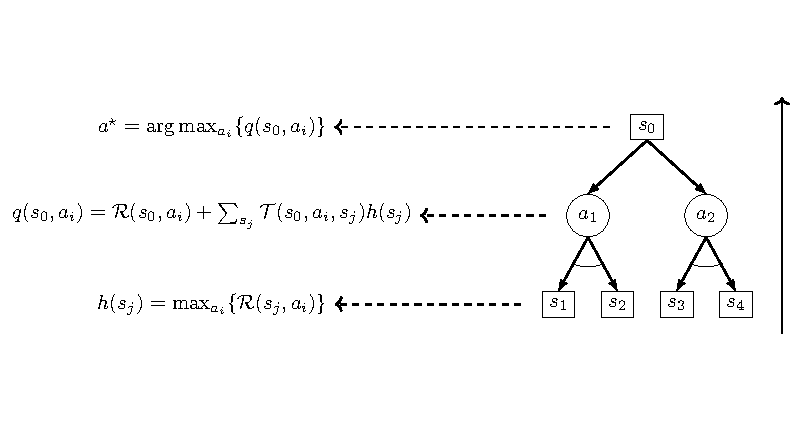
\includegraphics[width=0.9\textwidth]{images/MasterThesisAndOrTree(1).pdf}
  \caption{Look-ahead search space, depth $D = 1$ (MDP)}
  \label{fig:tree}
\end{figure}
\item The execution phase consists in executing the action, say $a^{\star}$, associated with the highest value estimate. The environment returns a new state $s'$ that may now be used as the root of the search tree during the following planning phase.
    \end{itemize}
    
    \item \textit{Hybrid Offline-Online} approximations: In 2006, \textit{Parquet et al.} \cite{articlepomh} propose three algorithms for POMDPs that combine the advantages of several \textit{online} (RTBSS \cite{rtbss}, RTDP-BEL \cite{rtdpbel}) and \textit{offline} algorithms ($Q_{MDP}$ \cite{qmdp}, PBVI \cite{Pineau-2003-8730}), and show that they can often outperform \textit{online} and \textit{offline} approaches alone. In 2011, \textit{Maniloff et al.} \cite{maniloff} introduce \textit{Hybrid Value Iteration} for POMDPs, an algorithm that combines PBVI and look-ahead (tree) search to meet real-time constraints. The heuristic tree search is thereby used to occasionally make improvements to the value function initially computed offline using PBVI.
\end{itemize}


\section{Relational representation of the state space}
\label{sec:repstat}
Thus far, states have been handled like elements with no apparent relations between them. Concretely, the state spaces were not described in terms of a set of features that apply to and make up its elements. Consequently, as the environments described become more complex and are made up of more features, the state spaces grow exponentially with the number of features \cite{masbook}, thus quickly leading to unmanageable transition models. It is worth briefly discussing ongoing research in the field of \textit{relational} decision-making.


Many real-world domains are inherently relational \cite{Nitti2017}. In particular, from a \textit{logic programming} point of view, the state space of an environment can be described by a collection of \textit{relations} that jointly make up the features of the state space \cite{bout2, rrmdp}, and the states are \textit{Herbrand interpretations} of said collection \cite{relationallogic}. As such, an environment that describes a blocks world could be made up of the relations \texttt{on/2} and \texttt{clean/1}, while a possible world, that is, a state could be \texttt{on(A,C)}, \texttt{clean(B)}, where \texttt{A}, \texttt{B}, and \texttt{C} represent blocks (the example is taken from \textit{Nitti et al.}, 2017 \cite{Nitti2017}). This state is schematized in \RefFig{fig:block}. Actions are then described as facts (e.g., \texttt{move(A,B)}), and the state transition model is modeled through probabilistic rules. In 2001, \textit{Boutilier et al.} \cite{bout2} introduced the first \textit{relational} (\textit{first-order}) MDP (RMDP) and provided an algorithm for solving RMDPs using the \textit{Bellman equations} called \textit{Symbolic Dynamic Programming}. This \textit{structured} approach to the representation of states makes it possible to solve complex (real-world) problems of relational nature, that is, problems in which states are made up of multiple features.




\begin{figure}[h]
\centering
    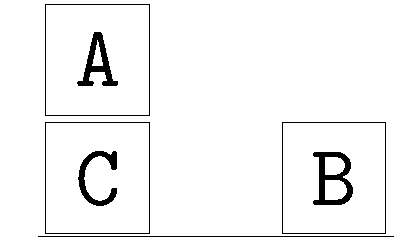
\includegraphics[width=0.25\textwidth]{images/MasterThesisRelationalDraw.pdf}
  \caption{A state of the blocks world}
  \label{fig:block}
\end{figure}


Note that, due to the simple nature of the scenarios discussed in later chapters, and given that the use of this representation is not indispensable to the study of the framework of interest of this thesis, we do not adopt a \textit{relational} approach for representing the states of the environment.

\chapter{Related work: Multi-agent formalisms}
\label{chap:related}
%\section{Aims}
%\label{sec:marl}
Multi-agent learning (MAL) problems are problems where an agent is to learn to behave optimally in the company of other agents, which may or may not be learning themselves \cite{Tuyls_Weiss_2012}.
Multi-agent settings are inherently more complex than their single-agent counterpart. In particular, several useful properties that hold in single-agent settings are no longer valid in multi-agent settings. Nevertheless, MAL techniques are used in practice and generally produce good results \cite{fundamentallymoredifficult}. \RefSec{sec:additional} addresses some of the challenges that arise when moving from a single-agent setting to a multi-agent setting. Sections \ref{sec:mmdp}, \ref{sec:decpomdp}, and \ref{sec:ipomdp} then summarize several multi-agent frameworks. Finally, \RefSec{sec:repnet} covers the multi-agent, POMDP-based framework called \textit{Reputation Network} POMDP.
\section{Challenges in multi-agent formalisms}
\label{sec:additional}
\subsection{Non-stationarity}
An intuitive and naive way of dealing with the presence of multiple agents from the perspective of one agent $g$ may be to consider every other agent to be a part of the environment. In fact, by assuming that each agent $h$ is following a stationary policy $\pi_h$, solving a MAL problem from the perspective of agent $g$ reduces to solving a single-agent problem where the behavior of all other agents is factored in the environment's transition model \cite{reduce, reduce2}. This assumption is not always reasonable and, more often than not, the agents will adapt their policy as time goes by \cite{nonstation}. Alongside the impossibility of reducing the problem, \textit{correlated goals} and the \textit{loss of convergence guarantee} discussed hereafter have a significant impact on multi-agent learning.

\subsection{Correlated goals}
In single-agent settings, the rewards collected by the agent are a function of the state of the environment. In multi-agent settings, a first consequence of the non-stationarity of policies is that one agent's returns will likely depend on the other agents' behavior as well \cite{nonstation}. Explicit modeling of the reward scheme may, therefore, be significantly more complex.

\subsection{The convergence problem}
Another consequence of the non-stationarity of policies is the invalidation of the convergence guarantee of most Single-agent learning (SAL) algorithms \cite{nonstation, convergence}. In fact, the convergence of one agent's policy is now a function of all other agents' behavior in the network.

\subsection{The curse of dimensionality}
In complexity theory, a problem is considered to suffer from the curse of dimensionality with respect to a variable $n$ if
\begin{align}
    \label{eq:intract}
    T(n) = \Omega(2^n),
\end{align}
where $\Omega$ is the lower-bound on complexity, and $T$ is the number of steps required to solve said problem \cite{cursedim2}. Such a problem is said to be \textit{intractable}. Multi-agent learning problems are not the only ones subject to the curse of dimensionality: in fact, \RefSec{sec:intract} already illustrated the intractability of solving classic single-agent POMDPs via \textit{Value Iteration}. The problem worsens considerably when moving to multi-agent frameworks \cite{cursedim}.


\section{Multi-agent MDP: A centralized framework}
\label{sec:mmdp}
The Multi-agent MDP (MMDP) was formalized by Boutilier in 1996 \cite{Boutilier}, and is one of the first and simplest multi-agent learning frameworks.
\begin{definition}[Multi-agent MDP]
\label{def:mmdp}
A multi-agent Markov Decision Process, or simply MMDP, $\mathcal{M}$ is formally defined as a tuple
\begin{align*}
    \mathcal{M} := \big \langle \mathcal{S}, \mathcal{G}, \mathcal{A} = \times_{g \in \mathcal{G}} \mathcal{A}_g, \mathcal{T}, \mathcal{R} \big \rangle
  \end{align*}
where:
\begin{itemize}
    \item $\mathcal{S}$ is the set of possible states of the environment.
    \item $\mathcal{G}$ is the set of agents that can interact with the environment.
    \item $\mathcal{A}_g$ is the set of actions available to agent $g$.
    \item $\mathcal{A}$ is the set of joint actions.
    \item $\mathcal{T} : \mathcal{S} \times \mathcal{A}_1 \times ... \times \mathcal{A}_n \times  \mathcal{S} \rightarrow [0,1]$ is called the \textit{transition model}. 
    \item $\mathcal{R}: \mathcal{S} \times \mathcal{A}_1 \times ... \times \mathcal{A}_n \rightarrow \R$ is called the \textit{team reward function}.
\end{itemize}
\end{definition}



MMDP agents are assumed to be \textit{fully cooperative} \cite{Boutilier}, that is, they have no individual motivation. Their sole goal lies in maximizing the global (i.e. shared) expected reward. Each agent is furthermore assumed to have \textit{individual full state observability}, meaning all agents observe the same state. One can, therefore, think of an MMDP as a \textit{joint-action} MDP in which a single, \textit{central} unit applies \textit{joint actions} to the environment \cite{oliehoek}. The \textit{joint-action} policy 
\begin{align}
    \pi : \mathcal{S} \rightarrow \mathcal{A},
\end{align}
associated with the shared value function $V^{\pi}$ is hereby to be maximized. Having a \textit{central} unit follow the present \textit{joint-action} policy is equivalent to having each agent $g$ follow their respective individual policy $\pi_g : \mathcal{S} \rightarrow \mathcal{A}_g$, derived from $\pi$ \cite{oliehoek}. As such, MMDPs are said to make up a \textit{centralized} framework.



\section{Decentralized-POMDP: Decentralized policy execution}
\label{sec:decpomdp}
A major assumption of MMDPs is that each agent is fully aware of the complete state of the environment, at all times. This assumption may not always be realistic \cite{decmdp}. In 2002, still in the realm of \textit{cooperative} planning, Bernstein et al. \cite{decmdp2} took a \textit{decentralized} approach to MDPs in multi-agent settings, by incorporating the idea of \textit{individual- or local- observations}, as well as having the agents be unaware of the other agents' \textit{observations}. This decentralization is fundamentally different to MMDPs and makes DEC-POMDPs more difficult to solve. It should be noted that, while the \textit{online} phase, i.e. execution of the learned plan, is, in fact, completely decentralized, the \textit{offline} phase, i.e., the actual planning, is centralized \cite{moredec}. More specifically, a single centralized unit computes the joint-action policy offline and then distributes the individual policies to be executed by the agents online.

\begin{definition}[DEC-POMDP]
\label{def:decpomdp}
A decentralized Partially Observable Markov Decision Process, or DEC-POMDP, $\mathcal{D}$ is formally defined as a tuple
\begin{align*}
    \mathcal{D} := \big \langle \mathcal{S}, \mathcal{G}, \mathcal{A} = \times_{g \in \mathcal{G}} \mathcal{A}_g, \Omega = \times_{g \in \mathcal{G}} \Omega_g, \mathcal{T}, \mathcal{R}, \mathcal{O} \big \rangle
  \end{align*}
where:
\begin{itemize}
    \item $\mathcal{S}$, $\mathcal{G}$, $\mathcal{A}_g$, $\mathcal{A}$, $\mathcal{T}$, and $\mathcal{R}$ are defined as in \RefDef{def:mmdp}.
    \item $\Omega_g$ is the set of observations available to agent $g$.
    \item $\Omega$ is the set of joint observations.
    \item $\mathcal{O} : \mathcal{A} \times \mathcal{S} \times \Omega \rightarrow [0,1]$ is called the \textit{joint observation function}.
\end{itemize}
\end{definition}
DEC-POMDPs can be reduced to DEC-MDPs if there exists a mapping $J$ such that
\begin{align}
    J: \Omega_1 \times ... \times \Omega_n \rightarrow S,
\end{align}
in other words, if the joint observation of all agents uniquely identifies the state of the environment. The state is then said to be \textit{jointly fully observable}. It is worth noting that even then, the agents themselves are only aware of their \textit{individual observations} \cite{oliehoek}.

\section{Interactive-POMDP: A framework for self-interested agents}
\label{sec:ipomdp}
In 2005, Gmytrasiewicz et al. formalized a further extension of POMDPs to multi-agent settings, called Interactive-POMDP \cite{ipomdp}. In contrast to MMDPs and DEC-POMDPs, I-POMDPs make no assumption about the willingness of the agents to be \textit{cooperative}. In fact, I-POMDPs are mainly applied to domains made up of \textit{autonomous} and \textit{self-interested} agents. While in DEC-POMDPs the optimal joint policy is computed by a \textit{centralized} unit before being distributed amid the agents, the self-interested nature of I-POMDP agents requires the \textit{learning} algorithms to be \textit{decentralized}, that is, each agent is to locally compute its own policy as a function of its beliefs about the physical state of the environment as well as its interactions with the other agents.

\begin{definition}[I-POMDP]
\label{def:decpomdp}
An Interactive Partially Observable Markov Decision Process, or I-POMDP, of an agent, say $g$, is written $\mathcal{I}_g$ and is formally defined as a tuple
\begin{align*}
    \mathcal{I}_g := \big \langle \mathcal{IS}_g, \mathcal{A} = \times_{g \in \mathcal{G}} \mathcal{A}_g, \Omega_g, \mathcal{T}_g, \mathcal{R}_g, \mathcal{O}_g \big \rangle
  \end{align*}
where:
\begin{itemize}
    \item $\mathcal{IS}_g : \mathcal{S} \times_{h:h \neq g} \mathcal{M}_h$ is the set of interactive states of agent $g$. Interactive states are physical environment states augmented with models of each agent in the network.
    \item $\mathcal{A}_g$ and $\mathcal{A}$ are defined as in \RefDef{def:mmdp}.
    \item $\Omega_g$ is the set of observations available to agent $g$.
    \item $\mathcal{T}_g : \mathcal{S} \times \mathcal{A} \times \mathcal{S} \rightarrow [0,1]$
    \item $\mathcal{R}_g : \mathcal{IS}_g \times \mathcal{A} \rightarrow \R$ is called the \textit{immediate} reward of agent $g$.
    \item $\mathcal{O}_g : \mathcal{A} \times \mathcal{S} \times \Omega_g \rightarrow [0,1]$ is called the \textit{observation function} of agent $g$.
\end{itemize}
\end{definition}
In accordance with the definition of \textit{interactive states}, I-POMDP agents update their beliefs not only over physical states of the environment but also over models of the other agents in the network. The difficulty of solving I-POMDPs lies in the recursive nature of the models. Consider agent $g$'s belief update in a network inhabited by another agent, say $h$. A model of agent $h$ may consist of the belief function of said agent $h$ over physical states and models of all other agents. These models may, in turn, consist of belief functions of their own. This nesting of beliefs could theoretically be infinite, rendering the belief update \textit{non-computable}. This inconvenience is overcome by bounding the nesting depth by a finite number $n$. The problem is then solved as a set of POMDPs. 

In 2009, \textit{Doshi et al.} \cite{monteipomdp} mitigate the computational requirements for solving I-POMDPs by using \textit{Monte Carlo Sampling Methods} to find approximate solutions. In 2011, the complexity of real-world \textit{interactive state spaces} is addressed; \textit{Panella et al.} \cite{impomdprel} introduce a new representation for \textit{interactive states} that draws from \textit{relational} (\textit{first-order}) logic and probability theory, in an attempt to compactly and finitely represent \textit{interactive state spaces}. Recently, in 2019, \textit{Han et al.} \cite{impomdpnn} introduce IPOMDP-Net, a framework that combines I-POMDPs and \textit{Deep Learning}. Their approach is shown to outperform \textit{state-of-the-art} model-free networks. Concretely, IPOMDP-Net is a \textit{deep neural network} that embeds an I-POMDP and a QMDP planner (\cite{qmdp}) in its network architecture.
\section{The RepNet-POMDP framework}
\label{sec:repnet}
This section introduces the multi-agent, POMDP-based framework called Reputation Network POMDP, which was proposed by \textit{Rens et al.} in their paper "\textit{Maximizing Expected Impact in an Agent
Reputation Network}" published in 2018 \cite{rensetal} and constitutes the foundation of the work presented in the rest of the thesis. Several multi-agent frameworks have been presented in this chapter. 

To highlight their differences from the RepNet framework, their domains of use are briefly revised here. MMDPs and DEC-POMDPs serve a similar purpose in that they are used to compute a global policy that maximizes the collective well-being of the agents that make up the framework. Consequently, said agents are assumed to be completely selfless. This heavily contrasts with the intended purpose of the RepNet framework, in which each agent uses its \textit{own} instance of the framework, and in which no assumption is made concerning their selflessness. I-POMDPs do serve a similar purpose as far as not making assumptions about an agent's selflessness. They are, however, arguably significantly more difficult to conceptualize than the framework presented hereafter. The RepNet framework achieves a more intuitive layout by making assumptions about the elements that should matter to the agents. In particular, agent \textit{reputation} and \textit{past behavior} of agents are key drivers of the interactions between the agents of the network.


The working principles of the framework are first introduced, after which its planning algorithm is detailed. Note that this section summarizes the framework in its entirety: a few concepts presented hereafter play a minor role in the remainder of this thesis. More concretely, the concepts of \textit{partial observability} and \textit{state estimation} will be worked out of the framework in \RefChap{chap:mdp}. The most important concepts of the framework will be reiterated when necessary in future chapters. 


\subsection{Presentation of the framework}
The \textit{RepNet} framework is aimed at solving multi-agent learning problems in which each agent is associated with a reputation in the network, and their reputation, as well as past behavior, dictate the willingness of the rest of the network to engage in communications with them. Similarly to classic POMDP systems, the rules of \textit{stochasticity} and \textit{partial observability} apply to the environments considered here.
Intuitively, the framework can be thought of as the combinations of 4 pillars.

    \paragraph{The underlying Markov Decision Process structure:} RepNet agents move about in a \textit{stochastic} environment characterized by a set of \textit{states}, and the rules of the environment are described in a \textit{transition model}. RepNet agents progress in the environment by applying one of the \textit{actions} at their disposal. The primary goal of RepNet agents is the \textit{maximization of its long-term cumulative reward}.
    
    \paragraph{A tracking mechanism of other agents' past behavior:} The actions taken by a RepNet agent are informed at all times by the past behavior of other agents in the network.
    
    \paragraph{A tracking mechanism of other agents' reputation:} Each agent has an opinion, be it good or bad, of the remaining agents in the network. RepNet agents explicitly monitor the image they \textit{believe} all agents to have of one another, and use this information in their decision-making process.
    
    \paragraph{A tracking mechanism of the environment's current potential states:} Analogously to Partially Observable Markov Decision Processes, RepNet agents are uncertain of the current state of the environment. Additionally, said agents monitor the state of the environment other agents believe to be in. 


\paragraph*{}The formal presentation of the framework follows hereafter.

\begin{definition}[RepNet-POMDP]\label{def:name}
Let $\Sigma$ be a tuple embedding global information about the system, i.e. the environment and agents that are part of said system, and $\Gamma$ be a tuple embedding each agent's subjective understanding of the environment it operates in. 
A \textit{reputation network POMDP} $\mathcal{M}$ is formally defined as a tuple
  \begin{align*}
    \mathcal{M} := \big \langle \Sigma, \Gamma \big \rangle.
  \end{align*}

\end{definition}

\begin{definition}[System]
\label{def:systempo}
A system $\Sigma$ is formally defined as a tuple
\begin{align*}
    \Sigma := \big \langle \mathcal{G}, \mathcal{S}, \mathcal{A}, \Omega, \mathcal{I}, \mathcal{U} \big \rangle
  \end{align*}
where:
\begin{itemize}
    \item $\mathcal{G}$ is the set of agents that can interact with the environment.
    \item $\mathcal{S}$ is the set of possible states of the environment.
    \item $\mathcal{A}$ is the set of possible actions, both \textit{directed} towards a particular agent and \textit{undirected}. Formally,
    \begin{align*}
    \mathcal{A} := \mathcal{A}^d \cup \mathcal{A}^u\\
    \mathcal{A}^d \cap \mathcal{A}^u := \varnothing
  \end{align*}
  Note that the concept of \textit{undirected actions} is identical to the concept of actions in classic MDPs. The concept of \textit{directed actions} will be discussed in greater detail in \RefSec{sec:dirr}.
  
  \item $\Omega$ is the set of observations.
  \item $\mathcal{I}: \mathcal{G} \times \mathcal{G} \times \mathcal{S} \times \mathcal{A} \rightarrow [-1,1]$ is called the \textit{impact function}. $\mathcal{I}(g,h,s,a)$ returns the impact on agent $g$ that is due to agent $h$ performing action $a$ in state $s$. This function can be thought of as analogous to a Markov Decision Process's immediate reward function $\mathcal{R}$.
  \item $\mathcal{U} : [0,1] \times [-1,1] \times [-1,1] \rightarrow [-1,1]$ is called the \textit{image update function}. Given a learning rate $\alpha$, a current value $v$, of the image on agent has of another agent, to be updated, and a new expected total impact $i$, of which the definition will be given shortly, $\mathcal{U}(\alpha, v, i)$ returns an updated value of the image $v'$.
\end{itemize}
\end{definition}


\begin{definition}[Agents]
\label{def:agentspo}
Let $\Gamma$ be a tuple embedding each agent's subjective understanding of the environment it operates in, such that
\begin{align*}
    \Gamma := \big \langle \{UT_g\}, \{DT_g\},\{O_g\}, \{AD_g\}, \{Img_g\}, \{B_g\} \big \rangle
  \end{align*}
where:
\begin{itemize}
    \item $UT_g : \mathcal{G} \times \mathcal{S} \times \mathcal{A}^u \times \mathcal{S} \rightarrow [0,1]$ is called the \textit{undirected transition model} of agent $g$. $UT_g(h,s,a,s')$ returns the probability of the environment transitioning from state $s$ to state $s'$ when undirected action $a$ is taken by agent $h$.
    \item $DT_g : \mathcal{G} \times \mathcal{S} \times \mathcal{A}^d \times \mathcal{S} \times [-1,1] \rightarrow [0,1]$ is called the \textit{directed transition model} of agent $g$. $DT_g(h,s,a_{h\rightarrow i},r_h,s')$ returns the probability of the environment transitioning from state $s$ to state $s'$ when agent $h$ performs directed action $a_{h\rightarrow i}$ towards another agent, say $i$, and has a reputation $r_h$ according to agent $g$.
    
    \item $O_g$ is called the \textit{observation function}, or \textit{sensor model}, of agent $g$. $O_g(h,a,s',o)$ returns the probability of agent $g$ making observation $o$ after agent $h$, which may or may not be the same as $g$, performs action $a$ and the environment transitions to state $s'$.
    \item $AD_g : \mathcal{G} \times \mathcal{S} \rightarrow \Delta(\mathcal{A})$ is called the \textit{action distribution} of agent $g$. $AD_g(h,s)$ returns a probability distribution over actions in $\mathcal{A}$ for agent $h$ in state $s$, according to agent $g$.
    \item $Img_g : \mathcal{G} \times \mathcal{G} \rightarrow [-1,1]$ is called the \textit{image function} of agent $g$. $Img_g(h,i)$ returns the image agent $i$ has of agent $h$ according to agent $g$.
    \item $B_g : \mathcal{G} \rightarrow \Delta(\mathcal{S})$ is called the \textit{belief state} of agent $g$. $B_g(h)$ (generally written $b_h^g$ hereafter to simplify the notation) returns the belief state of agent $h$, according to agent $g$.
\end{itemize}
\end{definition}
The image two agents have of each other is conditioned by the \textit{impact} they are expected to have on each other, given their current understanding of the state the environment is in. The notion of expected total impact is formalized in \RefDef{def:imppo}, while its effect on the image function is defined in \RefDef{def:imgb}.
\begin{definition}[Expected total impact]
\label{def:imppo}
According to agent $g$, the total impact an agent $h$ is expected to have on, as well as perceive from, another agent $i$, assumed to be different from $h$, given current belief state function $B_g$ and action distribution function $AD_g$, is defined as
\begin{align*}
    ETI_{g} (h, i, B_g, AD_g) := &\sum_{s \in \mathcal{S}} b_h^g(s) b_i^g(s) \sum_{a \in \mathcal{A}} \, \big[ \, \delta AD_g(i, s)(a) \mathcal{I}(h, i, s, a)  \\&+ (1 - \delta) AD_g(h, s)(a) \mathcal{I}(i, h, s, a) \, \big]
\end{align*}
where $\delta \in [0,1]$ trades off the relative importance of the impact due to agent $h$ and the impact perceived by $h$.
\end{definition}

%\textcolor{red}{PROVE ETI $\in [-1,1]$ }

\begin{definition}[Image update]
\label{def:imgb}
Let $Img_g$ be the current image function of agent $g$. The updated image function $Img_g'$ is computed as follows:
\begin{align*}
     Img_g' &:= IE(g,Img_g,\alpha, B_g, AD_g) \\&:= \Big\{(h,i, t) \,\,\Big| \,\,h,i \in \mathcal{G} \land t =  \mathcal{U}(\alpha, Img_g(h,i), ETI_{g}(h, i,B_g, AD_g)) \Big\}
\end{align*}
where
\begin{itemize}
    \item $IE$ is called the \textit{image estimation function}.
    \item $\alpha$ is called the learning rate.
    \item $B_g$ is the current belief state of agent $g$.
    \item $AD_g$ is the current action distribution of agent $g$.
\end{itemize}
\end{definition}

The reputation of an agent, say $h$, as defined by \textit{Rens et al.} \cite{rensetal}, brings together the image each agent has of $h$ as well as the image the RepNet agent of interest $g$ has of all the agents that make up the network. The mathematical definition is given in \RefDef{def:reppo}.

\begin{definition}[Reputation]
\label{def:reppo}
The reputation of an agent $h$, according to agent $g$, is formally defined as 
\begin{align*}
     REP_g(h, Img_g) := \frac{1}{|\mathcal{G}|} \sum_{i \in \mathcal{G}} Img_g(h,i) \times Img_g(i,g)
\end{align*}
where $Img_g(i,i) = 1 \,\,\forall i \in \mathcal{G}$.
\end{definition}

To simplify the notation, it is convenient to define a \textit{global transition model} that combines both directed and undirected transition models. The behavior of the new function should be dictated by the nature of the action passed as an argument to it.

\begin{definition}[Global transition model]
\label{def:globtran}
The global transition model of agent $g$, $T_g : \mathcal{G} \times \mathcal{S} \times \mathcal{A} \times \mathcal{S} \times [-1,1] \rightarrow [0,1]$, is formally defined as
\begin{align*}
     T_g(h, s,a_h,s', r_h) := 
    \begin{cases}
    DT_g(h, s,a_h,s', r_h) & \mbox{if } a_h \in \mathcal{A}^d
    \\
    UT_g(h,s,a_h,s') & \mbox{if } a_h \in \mathcal{A}^u
    \end{cases}
\end{align*}
where 
\begin{itemize}
    \item $h$ is the sender of action $a$.
    \item $a_h$ is the action, directed or undirected, taken by agent $h$.
    \item $s$ is the current state of the environment.
    \item $s'$ is the potential future state of the environment. Note that this state may be the same as state $s$.
    \item $r_h$ is the reputation of agent $h$, according to agent $g$.
\end{itemize}
\end{definition}

RepNet agents are uncertain of the state of the environment. Keeping track of a probability distribution over all possible states of the environment assists them in the decision-making process. Additionally, the partial observability that applies to them also applies to every agent in the network. Monitoring the state of the environment that the \textit{other} agents in the network believe to be in has the purpose of helping RepNet agents make better-informed decisions.

An agent's \textit{own} belief state, called \textit{objective belief state} hereafter, changes as it takes actions and makes new observations on the environment. The belief state update, defined in \RefDef{def:ose}, is analogous to that performed in classic POMDP problems (Equation \ref{eq:belief}).
\begin{definition}[Objective state estimation]
\label{def:ose}
Let $b_g^g$ be the current belief state of agent $g$ according to itself, or objective belief state of agent $g$. The updated objective belief state ${b_g^g}'$ is computed as follows:
\begin{align*}
    {b_g^g}' 
    &:= OSE(b_g^g, a, g, o, r_g) \\
    &:= \Bigg\{(s', p) \,\,\Bigg| \,\,s'\in \mathcal{S} \land p = \frac{ O_g(g,a,s',o) \sum_{s} T_g(g,s,a,s', r_g)b_g^g(s)}{P_g(o | b_g^g,a,g,r_g)} \Bigg\}
\end{align*}
where:
\begin{itemize}
    \item $OSE$ is called the \textit{objective state estimation function}.
    \item $a$ is the action taken by agent $g$.
    \item $o$ is the observation made by agent $g$ after taking action $a$.
    \item $r_g$ is the reputation of agent $g$, according to itself.
    \item $P_g(o | b_g^g,a,g,r_g) = \sum_{s'} O_g(g,a,s',o) \sum_{s} T_g(g,s,a,s', r_g)b_g^g(s)$ is a normalizing constant.
\end{itemize}
\end{definition}
Alongside its own belief state, each agent has an idea of what state other agents in the network believe the environment to be in. This information is maintained in so-called \textit{subjective belief states}, which, similarly to their objective counterparts, are updated upon receiving new observations. The update of subjective belief states is defined in \RefDef{def:sse}.
\begin{definition}[Subjective state estimation]
\label{def:sse}
Let $b_h^g$ be the current belief state of agent $h$ according to agent $g$. The updated subjective belief state ${b_h^g}'$ is computed as follows:
\begin{align*}
    {b_h^g}' &:= SSE(b_h^g, AD_g,h, o, r_h) \\&:= \Bigg\{(s', p) \,\,\Bigg| \,\, s'\in \mathcal{S} \land p =  \frac{\sum_{a}O_g(h,a,s',o) \sum_{s} T_g(h,s,a,s',r_h) b_h^g(s) AD_g(h,s)(a)}{P_g(o | b_h^g,h,o,r_h,AD_g)} \Bigg\}
\end{align*}
where:
\begin{itemize}
    \item $SSE$ is called the \textit{subjective state estimation function}.
    \item $o$ is the observation made by agent $g$.
    \item $r_h$ is the reputation of agent $h$, according to agent $g$.
    \item $P_g(o | b_h^g,h,o,r_h,AD_g) = \sum_{s'}\sum_{a }O_g(h,a,s',o) \\\cdot\sum_{s} T_g(h,s,a,s',r_h) b_h^g(s) AD_g(h,s)(a)$ is a normalizing constant.
\end{itemize}
\end{definition}

The concepts of \textit{objective} and \textit{subjective} state estimation can now be combined into a single concept called \textit{total state estimation}.

\begin{definition}[Total state estimation]
Let $B_g$ be the current belief state function of agent $g$, and $o$ is the observation made by agent $g$ after taking action $a$. The updated belief state function $B_g'$ is computed as follows:
\begin{align*}
    B_g' &:= SE(g,B_g,a,o, Img_g, AD_g) \\&:=  \Big\{(h, SSE(b_h^g, AD_g, h, o, r_h)) \,\,\Big| \,\, h\in \mathcal{G} \setminus \{ g \} \land r_h = REP_g(h, Img_g) \Big\} \\
    & \,\,\,\,\,\,\,\,\,\,\cup \Big\{(g, OSE(b_g^g, a, g, o, REP_g(g, Img_g)))  \Big\}
\end{align*}
where $SE$ is called the \textit{total state estimation function}.
\end{definition}

The next step in the formalization of RepNet-POMDPs consists in defining an updating scheme of the action distribution $AD_g$ of each agent $g$. \textit{Rens et al.} \cite{rensetal} propose a model based on Bayesian conditioning.\\
A Bayesian agent $g$ updates its subjective experience of the world it operates in light of new information. Say an environment hosting two agents $g$ and $h$ is currently in state $s$. Agent $g$ has an \textit{a priori} idea of the probability of agent $h$ picking an action $a$ in state $s$,
\begin{align}
    P_g(a | h, s, r_h).
\end{align}
Following agent $h$ performing action $a$ in this state, the environment transitions from state $s$ to a new unknown state. The observation $o$ agent $g$ makes can be used by said agent to update its subjective perception of the \textit{a posteriori} probability of agent $h$ performing that same action $a$ in state $s$ in the future, using Bayes' theorem\footnote{Bayes' theorem is defined mathematically as follows: $P(A | B,C) = \frac{P(B|A,C) P(A|C)}{P(B|C)}$, where $A$, $B$ and $C$ are events and $P(B | C) \neq 0$},
\begin{align}
\label{eq:34}
\begin{split}
    P_g(a | h,s,r_h,o) &= \frac{P_g(o | h,s,r_h,a) P_g(a | h, s,r_h)}{P_g(o|h,s,r_h)} 
    \\
    &= \frac{P_g(o | h,s,r_h,a) P_g(a | h, s)}{\sum_{a'} P_g(o|h,s,r_h,a') P_g(a' | h,s)}
\end{split}
\end{align}
where $P_g(o | h,s,r_h,a)$ is calculated as follows:
\begin{align}
\begin{split}
    P_g(o | h,s,r_h,a) &= \sum_{s' \in \mathcal{S}} P_g(o | h,s,r_h,a,s') P_g(s' | h,s,r_h,a) \\&= \sum_{s' \in \mathcal{S}} O_g(h,a,s',o) T_g(h,s,a,s',r_h)
    \end{split}
\end{align}

The probabilities in Equation \ref{eq:34} can now be replaced by the terms defined in \RefDef{def:agentspo} and \RefDef{def:globtran}:
\begin{align}
    P_g(a | h,s,r_h,o) = \frac{\sum_{s'} T_g(h,s,a,s',r_h) O_g(h,a,s',o) AD_g(h,s)(a)}{\sum_{a'} \sum_{s'} T_g(h,s,a',s',r_h) O_g(h,a',s',o) AD_g(h,s)(a')}.
\end{align}

\begin{definition} [Action distribution update]
\label{def:actup2}
Let $AD_g$ be the current action distribution function of agent $g$. The updated action distribution $AD_g'$ is computed as follows:
\begin{align*}
     AD_g' &:= ADE(g, o, AD_g, Img_g) \\&:= \Bigg\{(h,s,a,p) \,\,\Bigg| \,\, h \in \mathcal{G} \land s \in \mathcal{S} \land a \in \mathcal{A} \,\land r_h = REP_g(h, Img_g)
     \\& \,\,\,\,\,\,\,\,\,\,\, \land p =  \frac{\sum_{s'} T_g(h,s,a,s',r_h) O_g(h,a,s',o) AD_g(h,s)(a)}{\sum_{a'} \sum_{s'} T_g(h,s,a',s',r_h) O_g(h,a',s',o) AD_g(h,s)(a')} \Bigg\}
\end{align*}
where
\begin{itemize}
    \item $ADE$ is called the \textit{action distribution estimation function}.
    \item $o$ is the observation made by agent $g$.
\end{itemize}
\end{definition}






\subsection{Transition model}
\label{sub:totaltrans}
While the notion of transition models is used throughout \textit{Rens et al.} \cite{rensetal}, the physical meaning of each agent's transition model and how these transition models relate to one another is not explained. This section summarizes the approach taken in this thesis by illustrating it with a simple example that involves 2 agents.

Let $A$ and $B$ be two agents deployed in an environment that can be in any of the states in $\mathcal{S} = \{s_0, s_1 \}$. Each agent can pick any of the actions in $\mathcal{A} = \{ a_0, a_1\}$. For the sake of keeping the scenario simple, $\mathcal{A} = \mathcal{A}^u$, that is, all actions are undirected. Agent $A$'s transition model is given by $UT_A(A, s, a, s')$, while Agent $B$'s is given by $UT_B(B, s, a, s')$. These models describe the rules the agents abide by. The current definition for these models does, however, not explain how these individual models relate to the actual working principles of the environment. To address this point, a \textit{transition model of the environment} $\mathcal{T}$ can be introduced: 
\begin{align}
    \mathcal{T} : \mathcal{S} \times \mathcal{A}_A \times \mathcal{A}_B \times  \mathcal{S} \rightarrow [0,1],
\end{align}
such that $\mathcal{A}_A = \mathcal{A}_B = \mathcal{A}$. This definition is akin to the definition of transition model for Multi-agent MDPs (\RefSec{sec:mmdp}) and Decentralized-POMDPs (\RefSec{sec:decpomdp}). The individual transition models are now obtained as follows:
\begin{align}
\begin{split}
    &UT_A(A, s_i, a_i, s_j) = \frac{1}{|\mathcal{A}_B|} \sum_{a' \in \mathcal{A}_B} \mathcal{T}(s_i, a_i, a', s_j)  \,\,\,\,\, \forall s_i, s_j \in \mathcal{S}, \forall a_i \in \mathcal{A}_A \\&
    UT_B(B, s_i, a_i, s_j) = \frac{1}{|\mathcal{A}_A|} \sum_{a' \in \mathcal{A}_A} \mathcal{T}(s_i, a', a_i, s_j)  
    \,\,\,\,\, \forall s_i, s_j \in \mathcal{S}, \forall a_i \in \mathcal{A}_B.
\end{split}
\end{align}
Note that with this approach, 
\begin{align}
\begin{split}
    &UT_A(A, s_i, a_i, s_j) = UT_B(A, s_i, a_i, s_j) \\& UT_B(B, s_i, a_i, s_j) = UT_A(B, s_i, a_i, s_j),
\end{split}
\end{align}
that is, the individual transition models are independent from the agent they belong to. In an effort to simplify the notation, the subscript identifying this agent is dropped henceforth.

The definition provided above can be generalized to $n$ agents.
Let $\mathcal{A}'$ be the set of all possible combinations of actions for each agent with the exception of Agent $i$, i.e.,
\begin{align}
    \mathcal{A}' = \mathcal{A}_{1} \times ... \times \mathcal{A}_{i-1} \times \mathcal{A}_{i+1} \times ... \times \mathcal{A}_{n}
\end{align}
Agent $i$'s individual transition model is obtained as follows:
\begin{align}
    UT(i, s_i, a_i, s_j) = \frac{1}{|\mathcal{A}'|} \sum_{a' \in \mathcal{A}'} \mathcal{T}(s_i, a_i, a', s_j)  \,\,\,\,\, \forall s_i, s_j \in \mathcal{S}, \forall a_i \in \mathcal{A}_i
\end{align}












\subsection{The concept of directed actions}
\label{sec:dirr}

%\label{sub:direct}

The present section covers the concept of \textit{directed actions}, as described by \textit{Rens et al.} \cite{rensetal}. It furthermore serves to point out a shortcoming in the current definition of directed action.
In their paper, \textit{Rens et al.} describe a trade between two agents $A$ and $B$. $A$ is the \textit{buyer}, and $B$ is the \textit{seller}. The environment is described by the set of states 
\begin{align}
    \mathcal{S} = \{s_0, a, r\},
\end{align}
where $s_0$ is the initial state, $a$, called the \textit{accept} state, is the state in which the trade transaction was successfully completed, and $r$, called the \textit{refuse} state, is the state in which the trade transaction was unsuccessful. The actions at the disposal of both agents is described by the set 
\begin{align}
    \mathcal{A} = \{\texttt{trade\_with\_B}, \texttt{accept}, \texttt{refuse}, \texttt{wait}\}.
\end{align}
For the sake of simplicity, the environment is assumed to behave \textit{deterministically}, i.e., the outcome of any one combination of actions of $A$ and $B$ is always the same. Formally,
\begin{align}
\begin{split}
    &\mathcal{T}(s_0, \texttt{trade\_with\_B}, \texttt{accept}, a) = 1 \\
    &\mathcal{T}(s_0, \texttt{trade\_with\_B}, \texttt{refuse}, r) = 1,
\end{split}
\end{align}
where $\mathcal{T}$ is the \textit{transition model of the environment}, as per \RefSec{sub:totaltrans}.
The transition model \textit{of the environment} is given in \RefFig{fig:dir1}.
    
\begin{figure}[h]
  \begin{center}
    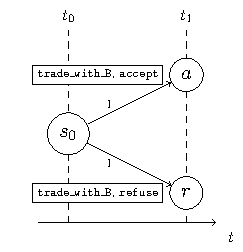
\includegraphics[width=0.4\textwidth]{images/MasterThesisDirectedActionsDraw (2).pdf}
  \end{center}
  \caption{Transition model $\mathcal{T}$ of the trading example. $s_0$ is the initial state, $a$ is the \textit{accept} state, and $r$ is the \textit{refuse} state. The transition model of the environment $\mathcal{T}$ is assumed to be deterministic.}\label{fig:dir1}
\end{figure}





At time $t_0$, agent $A$ performs action \texttt{trade\_with\_B} in state $s_0$. According to \textit{Rens et al.}'s definition of directed actions, the \textit{directed} probability of landing in state $a$ or $r$ at time $t_1$ is conditioned by the reputation of $A$, the agent initiating the trade. 
Consider the following situation: at time $t_0$ agent $A$ has a reputation of $0.5$, which is considered to be relatively good. The probability of $B$ being willing to trade with $A$ is, say, $0.9$, that is,
    \begin{align}
    \label{eq:transitions}
    \begin{split}
        &DT(A, s_0, \texttt{trade\_with\_B}, a, 0.5) = 0.9  \\&  DT(A, s_0, \texttt{trade\_with\_B}, r, 0.5) = 0.1. 
    \end{split}
    \end{align}
Said differently, at time $t_0$, agent $B$ will select action \texttt{accept} with a probability of $0.9$, and action \texttt{refuse} with a probability of $0.1$. 
The problem with the interpretation of the concept of directed actions by \textit{Rens et al.} is twofold:
\begin{itemize}
    \item The first problem resides in the fact that agent $B$ is not aware of agent $A$'s desire to trade at time $t_0$, as agent $A$ has not yet performed \texttt{trade\_with\_B}. Said differently, agent $B$ has no reason to prefer \texttt{accept} over \texttt{refuse} at this point in time.
    \item Suppose now that agent $B$ is made aware of the action agent $A$ is about to perform at $t_0$. The second problem relates to the fundamental properties of transition models. A transition model describes the rules the environment abides by, that is, it explains how the environment reacts \textit{on the basis of the actions taken} by its actors. To move the environment from $s_0$ to $a$, agents $A$ and $B$ need to commit to actions \texttt{trade\_with\_B} and \texttt{accept} respectively. \textit{Directed} transition models fail to be able to describe the rules of the environment. To illustrate the problem clearly, the cases in which $B$ has committed to action \texttt{accept} and in which it has not yet done so will be considered separately: 
    \begin{itemize}
        \item \textbf{Agent $B$ has committed to action \texttt{accept}: }If both agents have committed to their respective actions, then the transitions can simply be explained using \textit{undirected} transitions, that is, transitions that do not depend on the reputation of any agent. As per \RefSec{sub:totaltrans}, the individual \textit{undirected} transitions that explain the rules of the environment as they pertain to agent $A$ are formally given by
        \begin{align*}
            \begin{split}
                UT(A, s_0, \texttt{trade\_with\_B}, a) &= \frac{1}{|\mathcal{A}|} \sum_{a' \in \mathcal{A}} \mathcal{T}(s_0, \texttt{trade\_with\_B}, a', a) 
                \\&= \frac{1}{4} (0 + 1 + 0 + 0) = \frac{1}{4}
                \\&= UT(A, s_0, \texttt{trade\_with\_B}, r)
            \end{split}
        \end{align*}
        
        \item \textbf{Agent $B$ has not yet committed to action \texttt{accept}: }If agent $B$ has not committed to an action yet, then the missing action makes it impossible to use the \textit{transition model of the environment} (\RefSec{sub:totaltrans}) as a basis for deriving the \textit{directed} transition models. Said differently, the directed transitions given in Equation \ref{eq:transitions} can not possibly describe the rules of the environment as they apply to agent $A$. At most, they describe agent $A$'s \textit{subjective} impression of the impact that its own reputation might have on the willingness of agent $B$ to accept its trade offer.
    \end{itemize}
\end{itemize}
A solution to both problems covered in this section will follow in \RefSec{sec:reimagined}.












\subsection{Planning for Optimal Impact}
In RepNet-POMDPs, an agent's ability to thrive in the network is reflected in the reputation it has in the eyes of the remaining agents. A good reputation for agent $g$ increases the likelihood of other agents being willing to \textit{cooperate} with $g$. Moreover, an agent should perform actions according to the \textit{perceived immediate impact} they have on itself.
\begin{definition}[Perceived immediate impact]
\label{def:perceivedpo}
The perceived immediate impact on agent $g$, written $PI_g$, is defined as
    \begin{align*}
        PI_g(B_g,AD_g, a) := &\frac{1}{|\mathcal{G}|} \sum_{s \in \mathcal{S}} b_g^g(s) \big[ \, \mathcal{I}(g,g,s,a) \\&+ \sum_{h \in \mathcal{G} \setminus \{ g \}}  \sum_{a' \in \mathcal{A}} \mathcal{I}(g, h, s, a') b_h^g(s) AD_g(h, s)(a') \, \big]
    \end{align*}
    where
    \begin{itemize}
        \item $a$ is the action performed by agent $g$.
        \item $AD_g$ is the current action distribution of agent $g$.
        \item $B_g$ is the current belief state of agent $g$.
        \item The first term describes the immediate self-impact as a consequence of agent $g$ performing action $a$.
        \item The second describes the expected immediate impact that the network, i.e., the remaining agents, has on agent $g$.
    \end{itemize}
\end{definition}


Analogously to classical POMDPs, a RepNet-POMDP agent $g$ strives to maximize its expected discounted perceived impact
\begin{align}
    \E \big[ \sum_{t = 0}^{k} \gamma^t PI_{g,t}\big]
\end{align}
where $\gamma$ is the \textit{discount factor} and $PI_{g,t}$ is agent $g$'s perceived immediate impact at time-step $t$. This is accomplished by computing the optimal value function $V_g$, as defined in \RefDef{def:optipo}.

\begin{definition} [Value function]
\label{def:optipo}
Let $V_g$ be the optimal value function of agent $g$ in a \textit{finite-horizon} setting. It satisfies the \textit{optimality equations}, which are defined as 
    \begin{align*}
        \begin{dcases}
            V_g(B_g, AD_g, Img_g, k) := &\max_{a \in \mathcal{A}} \Big\{ PI_g(B_g,AD_g,a) \\&+ \gamma \sum_{o \in \Omega} P_g(o | B_g, AD_g, Img_g, a) V_g(B_g', AD_g', Img_g', k-1) \Big\}  
            \\
            V_g(B_g, AD_g, Img_g, 1) := &\max_{a \in \mathcal{A}} \Big\{ PI_g(B_g,AD_g,a) \Big\} 
        \end{dcases}
    \end{align*}
    where
    \begin{itemize}
        \item $B_g' = SE(g, B_g, a, o, Img_g, AD_g)$.
        \item $AD_g' = ADE(g, o, AD_g, Img_g)$.
        \item $Img_g' = IE(g, Img_g, \alpha, B_g, AD_g)$.
        \item $\gamma \in [0,1]$ is called the \textit{discount factor}.
        \end{itemize} 
        
        $P_g(o | B_g, AD_g, Img_g, a)$ can be reformulated using the concepts of observation function, transition model, and belief state (note that the development that follows was left out of Rens et al.'s original paper \cite{rensetal}):
        \begin{align*}
         P_g(o | B_g, AD_g, Img_g, a) &= \sum_{s' \in \mathcal{S}} P_g(o | B_g, AD_g, Img_g, a, s') P_g(s' | B_g, AD_g, Img_g, a)
    \\
    &= \sum_{s' \in \mathcal{S}} P_g(o | a, s') \sum_{s \in \mathcal{S}} P_g(s' | a, s) P_g(s | B_g, AD_g, Img_g, a)
    \\
    &= \sum_{s' \in \mathcal{S}} O_g(g,a, s', o) \sum_{s \in \mathcal{S}} T_g(g, s, a, s',r_g) b_g^g(s)
    \end{align*}



    
\end{definition}
\begin{definition}[Optimal policy]
Let $B_g$ be the current belief state function, $AD_g$ the current action distribution, $Img_g$ the current image function of agent $g$, and $k$ the current horizon. The optimal action for agent $g$, written $\pi(B_g, AD_g, Img_g, k)$, is defined as
\begin{align*}
    \pi(B_g, AD_g, Img_g, k) := &\arg \max_{a \in \mathcal{A}} \Big\{ PI_g(B_g,AD_g,a) \\&+ \gamma \sum_{o \in \Omega} P_g(o | B_g, AD_g, Img_g, a) V_g(B_g', AD_g', Img_g', k-1) \Big\}.
\end{align*}
\end{definition}


\chapter{The RepNet-MDP framework}
\label{chap:mdp}
The primary goal of this thesis is to study the properties of the RepNet framework. More concretely, the concepts of \textit{action distribution}, \textit{image}, \textit{reputation}, and \textit{directed actions}, as well as their impact on RepNet agents' behavior are key elements that distinguish it from classic (Partially Observable) Markov Decision Processes. While the notion of \textit{partial observability} for RepNet agents differs slightly from the definition employed by POMDP agents, in that RepNet agents have to keep track of the state in which other agents believe to be in addition to their own belief, it is arguably the feature that separates RepNet-POMDPs the least from other MDP-derived frameworks. In an attempt to bring the RepNet framework closer to \textit{tractability} and simplify the study of its properties, it can be reduced from its POMDP setting to a fully observable setting. Several adjustments, covered in \RefSec{sec:reduct}, are necessary to make the starting framework \textit{fully observable}. 
Further alleviation of the \textit{intractability} of the framework can be achieved by favoring approximate solutions of satisfactory quality over exact solutions. To this end, a look-ahead-based approach similar to that described in the context of classic MDPs in \RefSec{sec:stateart} can be taken.

This chapter follows the following structure: \RefSec{sec:reduct} describes the steps necessary to reduce the RepNet framework to a fully observable setting and follows with the presentation of the reduced framework. \RefSec{sec:reimagined} provides a solution to the concept of \textit{directed actions} imagined by \textit{Rens et al.} \cite{rensetal}. \RefSec{sec:revv} reviews the concept of \textit{action distribution estimation} in fully observable settings. \RefSec{sec:planningoptimal} then discusses planning for optimal impact in the context of RepNet-MDPs. \RefSec{sec:onlineplan} introduces the online look-ahead algorithm used to further alleviate the intractability of the reduced RepNet framework. Finally, \RefSec{sec:genn} briefly reviews the mathematical definition of \textit{reputation}.


%\section{Intractability of the RepNet-POMDP framework}
%\label{sec:intrapo}

\section{Reduction of the RepNet-POMDP framework}
\label{sec:reduct}
A RepNet-MDP is, analogously to its POMDP counterpart (\RefDef{def:name}), defined as a tuple
\begin{align*}
    \mathcal{M} := \big \langle \Sigma, \Gamma \big \rangle.
  \end{align*}
where $\Sigma$ is the \textit{system} tuple and $\Gamma$ is the \textit{agents} tuple. Several adjustments are necessary to make the starting framework fully observable. 
\begin{itemize}
    \item The system as defined in \RefDef{def:systempo} includes the set of possible observations $\Omega$. Given that neither impact function $\mathcal{I}$ nor update function $\mathcal{U}$ make use of $\Omega$, it may be removed without further ramifications in the new definition of the system (\RefDef{def:system}).
    \item The agents that make up $\Gamma$ in \RefDef{def:agentspo} notably each have their own observation function $O_g$, which furthermore appears in several equations: 
    \begin{enumerate}
        \item Each agent $g$'s subjective perception of the world is maintained in the functions $AD_g$, $Img_g$, and $B_g$. The update of these concepts is conditioned by the observations it makes.
        \item The optimality equations (\RefDef{def:optipo}) sum over all possible observations, after which the recursive calls to the value function are weighted using the observation function.
    \end{enumerate}
    In a fully observable environment, each agent is completely aware of the current state of the environment, rendering the belief state function $B_g$ of each agent $g$ futile. More specifically,
    \begin{enumerate}
        \item Each agent $g$'s image function $Img_g$ is updated partly on the basis of $g$'s current belief function, as it appears in the expected total impact function (\RefDef{def:imppo}).
        \item The perceived immediate impact on agent $g$ (\RefDef{def:perceivedpo}) is likewise conditioned by its current belief state function $B_g$, and is simplified in the reduced framework.
        \item The recursive calls in the optimality equations are weighted by the agent's current belief state function.
    \end{enumerate}
\end{itemize}

\begin{definition}[RepNet-MDP system]
\label{def:system}
A system in a RepNet-MDP $\Sigma$ is formally defined as a tuple
\begin{align*}
    \Sigma := \big \langle \mathcal{G}, \mathcal{S}, \mathcal{A}, \mathcal{I}, \mathcal{U} \big \rangle
  \end{align*}
where $\mathcal{G}$, $\mathcal{S}$, $\mathcal{A}$, $\mathcal{I}$, and $\mathcal{U}$ are defined as in \RefDef{def:systempo}.
\end{definition}

\begin{definition}[Agents]
\label{def:agents}
Let $\Gamma$ be a tuple embedding each agent's subjective understanding of the environment it operates in, such that
\begin{align*}
    \Gamma := \big \langle \{UT_g\}, \{DT_g\}, \{AD_g\}, \{Img_g\} \big \rangle
  \end{align*}
where $UT_g$, $DT_g$, $AD_g$, and $Img_g$ are defined as in \RefDef{def:agentspo}.
\end{definition}

The updated definition of \textit{expected total impact} is given in \RefDef{def:imp}, while its effect on the \textit{image function} is given in \RefDef{def:img}.
\begin{definition}[Expected total impact]
\label{def:imp}
According to agent $g$, the total impact an agent $h$ is expected to have on, as well as perceive from, another agent $i$, assumed to be different from $h$, when the environment is in state $s$, is defined as
\begin{align*}
    ETI_{g} (h, i, s, AD_g) :=  \sum_{a \in \mathcal{A}} \, \big[ \, \delta AD_g(i, s)(a) \mathcal{I}(h, i, s, a)  + (1 - \delta) AD_g(h, s)(a) \mathcal{I}(i, h, s, a) \, \big]
\end{align*}
where $\delta \in [0,1]$ trades off the relative importance of impact due to agent $h$ and impact perceived by $h$.
\end{definition}

\begin{definition}[Image update]
\label{def:img}
Let $Img_g$ be the current image function of agent $g$. The updated image function $Img_g'$ is computed as follows:
\begin{align*}
     Img_g' &:= IE(g,Img_g,\alpha, s, AD_g) \\&:= \Big\{(h,i, t) \,\,\Big| \,\,h,i \in \mathcal{G} \land t =  \mathcal{U}(\alpha, Img_g(h,i), ETI_{g}(h, i,s, AD_g)) \Big\}
\end{align*}
where
\begin{itemize}
    \item $IE$ is called the \textit{image estimation function}.
    \item $\alpha$ is called the learning rate.
    \item $s$ is the current state of the environment.
\end{itemize}
\end{definition}

The mathematical definition of reputation for RepNet-POMDPs (\RefDef{def:reppo}), given by
\begin{align}
    REP_g(h, Img_g) := \frac{1}{|\mathcal{G}|} \sum_{i \in \mathcal{G}} Img_g(h,i) \times Img_g(i,g),
\end{align}
can produce undesirable results in regards to self-reputation. To demonstrate this, consider a scenario in which two agents, say $A$ and $B$, are deployed in an environment without ever having been in contact with one another. Their image of each other can, therefore, be assumed neutral, i.e.,
\begin{align}
    Img_A(B, A) = 0, \,\,\,\,\,\,\,\, Img_A(B,A) = 0.
\end{align}
At this point, the desired reputation-related numbers should show that agent $A$ believes every agent's reputation, including its own, to be neutral. While this is indeed the case for agent $B$'s reputation, the same does not apply to agent $A$'s self-reputation. In fact,
\begin{align*}
\label{eq:selfrep2}
    REP_A(A, Img_A) &= \frac{1}{2} \,\, \big[ Img_A(A,B) \times Img_A(B,A) + Img_A(A,A) \times Img_A(A,A) \big]
    \\&= \frac{1}{2} \,\, \big[ 0 + 1\big] = \frac{1}{2}.
\end{align*}
As such, agent $A$ believes itself to initially have a higher reputation than agent $B$. The definition of reputation that follows was adjusted to address this inconvenience.


\begin{definition}[Adjusted Reputation]
\label{def:repnew}
The reputation of an agent $h$, according to agent $g$, is formally defined as 
\begin{align*}
      REP_g(h, Img_g) := 
    \begin{cases}
    \frac{1}{|\mathcal{G}|} \sum_{i \in \mathcal{G}} Img_g(h,i) \times Img_g(i,g) & \mbox{if } h \neq g
    \\
    \frac{1}{|\mathcal{G}|-1} \sum_{i \in \mathcal{G} \setminus \{ g \}} Img_g(h,i) \times Img_g(i,g) & \mbox{otherwise}
    \end{cases}
\end{align*}
where $Img_g(i,i) = 1 \,\,\forall i \in \mathcal{G}$.
\end{definition}





\section{Reimagined concept of directed actions}
\label{sec:reimagined}
In \RefSec{sec:dirr}, the concept of \textit{directed} transitions, as it was developed by \textit{Rens et al.} \cite{rensetal}, was covered. Using a trading example between two agents, of which the transition model of the environment $\mathcal{T}$ is repeated in \RefFig{fig:dir15}, two problems were identified.


\begin{figure}[h]
  \begin{center}
    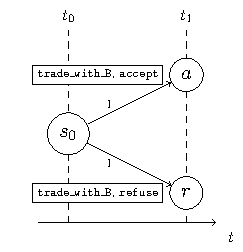
\includegraphics[width=0.4\textwidth]{images/MasterThesisDirectedActionsDraw (2).pdf}
  \end{center}
  \caption{Transition model $\mathcal{T}$ of the trading example. $s_0$ is the initial state, $a$ is the \textit{accept} state, and $r$ is the \textit{refuse} state. The transition model of the environment $\mathcal{T}$ is assumed to be deterministic.}\label{fig:dir15}
\end{figure}



The first problem resides in the fact that agent $A$ has not yet performed action \texttt{trade\_with\_B} at time $t_0$ and, as such, agent $B$ is not aware of $A$'s intentions. Concretely, there is no incentive for agent $B$ to favor action \texttt{accept} over action \texttt{refuse} at $t_0$. This problem is easily addressed by adding an \textit{intermediate} state $s_1$, in which agent $B$ is made aware of agent $A$'s desire to trade, to the transition model of the environment, and by rearranging the combinations of actions between any two states. The transition model with the intermediate state added is given in \RefFig{fig:dir2}.

\begin{figure}[h]
  \begin{center}
    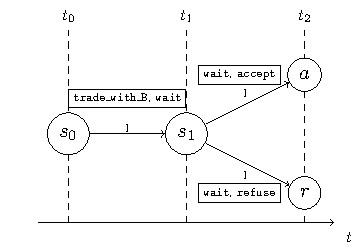
\includegraphics[width=0.6\textwidth]{images/MasterThesisDirectedNewDraw (2).pdf}
  \end{center}
  \caption{Updated transition model $\mathcal{T}$ of the trading example, $s_1$ is the state in which Agent $B$ is made aware of the trade offer.}\label{fig:dir2}
\end{figure}

The second problem pertains to the fact that \textit{directed} transition models can not describe the actual rules of the environment. In the case of the trade between agents $A$ and $B$, they can, at most, describe agent $A$'s \textit{subjective} impression of the impact that its own reputation might have on the willingness of agent $B$ to accept its trade offers. 
As such, one must make a clear distinction between the purpose of an \textit{undirected} transition model, which describes the actual rules of the environment as they apply to a single agent, and that of a \textit{directed} transition model, which describes that agent's \textit{subjective} perception of the rules of the environment. A version of the trading scenario between agents $A$ and $B$ that was adapted to make use of the concept of directed actions is presented hereafter.

The environment is made up of the same set of states $\mathcal{S} = \{s_0, s_1, a, r\}$ depicted in \RefFig{fig:dir2}. The set of \textit{undirected} actions at the disposal of both agents is given by
\begin{align}
    \mathcal{A}^u = \{\texttt{trade\_with\_B}, \texttt{accept}, \texttt{refuse}, \texttt{wait}\}.
\end{align}
\textit{In the eyes of} agent $A$, agent $B$'s response to a trade offer depends on $A$'s reputation. Concretely, $s_1 \rightarrow a$ and $s_1 \rightarrow r$
make up the transitions for which agent $A$ believes its reputation to be relevant. The action taken by agent $A$ during these transitions is \texttt{wait}. To make use of the notion of directed actions, the set of \textit{directed} actions $\mathcal{A}^d$ will contain the equivalent of \texttt{wait} in its \textit{directed} form, that is,
\begin{align}
    \mathcal{A}^d = \{\texttt{wait\_d}\}.
\end{align}

The way agent $A$ makes use of actions in $\mathcal{A}^u$ and $\mathcal{A}^d$ can now be detailed.
When reasoning about the value of each action, that is, when \textit{planning} to maximize its expected impact, agent $A$ will make use of \textit{undirected} actions in $\mathcal{A}^u$ whenever the action currently investigated has no equivalent in $\mathcal{A}^d$. For instance,
    \begin{align}
        T_A(A, s_0, \texttt{trade\_with\_B}, s_1, r_A) = UT(A, s_0, \texttt{trade\_with\_B}, s_1).
    \end{align}
    When an action in $\mathcal{A}^u$ has an equivalent in $\mathcal{A}^d$, agent $A$ will make use of the concept of directed actions in planning to maximize its expected impact. For instance,
    \begin{align}
        T_A(A, s_1, \texttt{wait}, a, r_A) = DT_A(A, s_1, \texttt{wait\_d}, a, r_A). 
    \end{align}
As such, the reputation of agent $A$ is accounted for when agent $A$ \textit{plans} to maximize its expected impact.
It is worth stressing that the rules of the environment do not change when agent $A$ reasons in terms of directed actions. Moreover, when agent $A$ is in $s_1$ and is to wait for agent $B$'s response to the trade offer, the action that is performed on the environment is the \textit{undirected} variant \texttt{wait}.










\section{Reviewing the action distribution estimation function}
\label{sec:revv}

The next step in the formalization of RepNet-MDPs consists in redefining the updating scheme of the action distribution $AD_g$ of each agent $g$. Initially, the reasoning applied here is similar to that applied to RepNet-POMDPs. Say an environment hosting two agents $g$ and $h$ is currently in state $s$. Agent $g$ has an \textit{a priori} notion of the probability of agent $h$ picking an action $a$ in state $s$,
\begin{align}
    P_g(a | h, s,r_h).
\end{align}
Following agent $h$ performing action $a$ in this state, the environment transitions from state $s$ to state $s'$. The \textit{a posteriori} probability of agent $h$ performing that same action $a$ in state $s$ in the future is now computed using Bayes' rule:
\begin{align}
\begin{split}
    P_g(a | h,s,r_h,s') &= \frac{P_g(s' | h,s,r_h,a) P_g(a | h, s,r_h)}{P_g(s'|h,s,r_h)} 
    \\
    &= \frac{P_g(s' | h,s,r_h,a) P_g(a | h, s)}{\sum_{a'} P_g(s'|h,s,r_h,a') P_g(a' | h,s)}.
\end{split}
\end{align}
The probabilities may now be replaced by the terms defined in \RefDef{def:agents} and \RefDef{def:globtran}:
\begin{align}
\label{eq:updateeq}
    AD_g'(h,s)(a) = \frac{T_g(h,s,a,s', r_h) AD_g(h,s)(a)}{\sum_{a'} T_g(h,s,a',s', r_h) AD_g(h,s)(a')}.
\end{align}




While MDP-derived formalisms are designed to deal with stochastic environments, one should expect them to work with deterministic transition models. The \textit{action distribution update} in \textit{fully observable} settings, as given in Equation \ref{eq:updateeq}, can produce undesirable results that make it impossible for a RepNet agent to \textit{unlearn} what it has learned.
Consider the trading scenario between agents $A$ and $B$ described in \RefSec{sec:reimagined} and whose transition model is schematized in \RefFig{fig:dir2}. The transitions of the environment are assumed to be deterministic, that is,
\begin{align}
    UT(B, s_1, \texttt{accept}, a) = 1, \,\,\,\,\, UT(B, s_1, \texttt{refuse}, r) = 1.
\end{align}
If agent $B$ refuses the trade offer made by agent $A$, the environment transitions to state $r$ and the action distribution is updated as follows:

\begin{align*}
    AD_A'(B,s_1)(\texttt{accept}) &=   \frac{UT(B,s_1, \texttt{accept},r) AD_A(B,s_1)(\texttt{accept})}{\sum_{a'} UT(B,s_1,a',r) AD_A(B,s_1)(a')}
    \\&=  \frac{0 \cdot AD_A(B,s_1)(\texttt{accept})}{\sum_{a'} UT(B,s_1,a',r) AD_A(B,s_1)(a')}
    \\&= 0
\end{align*}

\begin{align*}
    AD_A'(B,s_1)(\texttt{refuse}) &=   \frac{UT(B,s_1, \texttt{refuse},r) AD_A(B,s_1)(\texttt{refuse})}{\sum_{a'} UT(B,s_1,a',r) AD_A(B,s_1)(a')}
    \\&=  \frac{1 \cdot AD_A(B,s_1)(\texttt{refuse})}{\sum_{a'} UT(B,s_1,a',r) AD_A(B,s_1)(a')}
    \\&= 1
\end{align*}



As dictated by the new action distribution, agent $A$ is, in the wake of a \textit{single} unsuccessful trade, convinced that agent $B$ will never accept any trade offer in the future. Moreover, the primary issue does not reside in the fact that agent $A$ was quick to make up its mind, but in the fact that it is now impossible for agent $A$ to change its strategy in the future. In fact, the probability of $B$ accepting a trade is 0, and regardless of what this value is multiplied by in the future, it will always remain 0. 

This inconvenience is addressed hereafter by applying a \textit{smoothing} technique called \textit{Laplace smoothing} \cite{laplacesmoothing}. Let $\mathbf{\theta} = \langle \theta_1, \theta_2, ..., \theta_d \rangle$, such that $\theta_i \in [0,1] \,\, \forall i$ and $\sum_{i} \theta_i = 1$, be the probabilities of a multinomial distribution with $d$ categories. The \textit{Laplace-smoothed} estimators of the probabilities are given by

\begin{align}
    \hat{\theta}_i = \frac{\theta_i + \eta}{\sum_i (\theta_i + \eta)} = \frac{\theta_i + \eta}{\sum_i \theta_i + d\eta},
\end{align}
where $\eta \in [0,1]$ is called the \textit{smoothing parameter}. If $\theta_i \gg \eta$, then $\hat{\theta}_i \simeq \theta_i$. If $\theta_i \ll \eta$, then $\hat{\theta}_i \simeq \frac{1}{d}$. The smoothing technique thus prevents probabilities of 0 from ever occurring. The same smoothing technique can be applied to the \textit{action distribution update} function, resulting in the following equation:

\begin{align}
\label{eq:adu}
    AD_g'(h,s)(a) = \frac{T_g(h,s,a,s', r_h) AD_g(h,s)(a) + \eta}{\sum_{a'} (T_g(h,s,a',s', r_h) AD_g(h,s)(a') + \eta)}.
\end{align}

The new definition of the \textit{action distribution estimation} function (\RefDef{def:actupnew}) takes this smoothing technique into account.

\begin{definition} [Adjusted Action distribution update]
\label{def:actupnew}
Let $AD_g$ be the current action distribution function of agent $g$. The updated action distribution function $AD_g'$ is computed as follows:
\begin{align*}
     AD_g' &:= ADE(g, s', AD_g, Img_g) \\&:= \Bigg\{(h,s,a,p) \,\,\Bigg| \,\, h \in \mathcal{G} \land s \in \mathcal{S} \land a \in \mathcal{A} \,\land r_h = REP_g(h,Img_g)
     \\& \,\,\,\,\,\,\,\,\,\,\, \land p =  \frac{T_g(h,s,a,s', r_h) AD_g(h,s)(a) + \eta}{\sum_{a'} (T_g(h,s,a',s', r_h) AD_g(h,s)(a') + \eta)} \Bigg\}
\end{align*}
where
\begin{itemize}
    \item $ADE$ is called the \textit{action distribution estimation function}.
    \item $s'$ is the state the environment transitions to.
    \item $\eta$ is the \textit{smoothing parameter}.
\end{itemize}
\end{definition}













\section{Planning for optimal impact}
\label{sec:planningoptimal}

Optimal behavior in the context of RepNet-MDPs may now be described. To simplify the notation in this as well as in later sections, a construct called \textit{epistemic state} is defined hereafter.
\begin{definition}[Epistemic state]
\label{def:know}
The epistemic state $\theta_g$ of agent $g$ is formally defined as a tuple
\begin{align*}
     \theta_g := \big \langle s,  AD_g, Img_g \big \rangle
\end{align*}
where 
\begin{itemize}
    \item $s$ is the current state of the environment.
    \item $AD_g$ is the current action distribution of agent $g$.
    \item $Img_g$ is the current image function of agent $g$.
    \item $\theta_g \in \Theta_g$, and $\Theta_g$ is called the \textit{epistemic state set}. This set contains every possible combination of physical states of the environment, action distributions, and image functions of agent $g$.
\end{itemize}
\end{definition}
As with RepNet-POMDPs, an agent should perform actions according to the \textit{perceived immediate impact} they have on the agent itself. 
\label{sec:optimal}
\begin{definition}[Perceived immediate impact]
The perceived immediate impact on agent $g$, written $PI_g$, is defined as
    \begin{align*}
        PI_g(s,AD_g, a) := \frac{1}{|\mathcal{G}|} \, \big[ \, \mathcal{I}(g,g,s,a) + \sum_{h \in \mathcal{G} \setminus \{ g \}}  \sum_{a' \in \mathcal{A}} \mathcal{I}(g, h, s, a') AD_g(h, s)(a') \, \big]
    \end{align*}
    where
    \begin{itemize}
        \item $a$ is the action performed by agent $g$.
        \item $AD_g$ is the current action distribution of agent $g$.
        \item The first term describes the immediate self-impact as a consequence of agent $g$ performing action $a$.
        \item The second describes the expected immediate impact that the network, i.e., the remaining agents, has on agent $g$.
    \end{itemize}
\end{definition}
Analogously to classical MDPs, a RepNet-MDP agent $g$ strives to maximize its expected discounted perceived impact
\begin{align}
    \E \big[ \sum_{t = 0}^{k} \gamma^t PI_{g,t}\big]
\end{align}
where $\gamma$ is the \textit{discount factor} and $PI_{g,t}$ is agent $g$'s perceived immediate impact at time-step $t$. This is accomplished by computing the optimal value function $V_g$, as defined in \RefDef{def:opti}.
\begin{definition} [Value function]
\label{def:opti}
Let $V_g : \Theta_g \times \N \rightarrow \R$ be the optimal value function of agent $g$ in a \textit{finite-horizon} setting. It satisfies the \textit{optimality equations}, which are defined as 
    \begin{align*}
        \begin{dcases}
            V_g(\theta_g, k) := \max_{a \in \mathcal{A}} \Big\{ PI_g(s,AD_g,a) + \gamma \sum_{s' \in \mathcal{S}} T_g(g,s,a,s',r_g) V_g( \theta_g', k-1) \Big\}  &\forall \theta_g \in \Theta_g
            \\
            V_g(\theta_g, 1) := \max_{a \in \mathcal{A}} \Big\{ PI_g(s,AD_g,a) \Big\} &\forall \theta_g \in \Theta_g
        \end{dcases}
    \end{align*}
    where:
    \begin{itemize}
    \item $\theta_g = \big \langle s, AD_g, Img_g \big \rangle$
        \item $\theta_g' = \big \langle s', AD_g', Img_g' \big \rangle = \big \langle s', ADE(g, s', AD_g, Img_g), IE(g, Img_g, \alpha, s, AD_g) \big \rangle$.
        \item $\gamma \in [0,1]$ is called the \textit{discount factor}.
        \item $r_g = REP_g(g, Img_g)$.
    \end{itemize}
\end{definition}
\begin{definition}[Optimal policy]
Let $\theta_g$ be the current epistemic state of agent $g$, and $k$ the current horizon. The optimal action for agent $g$, written $\pi(\theta_g, k)$, is defined as
\begin{align*}
    \pi(\theta_g, k) := \arg \max_{a \in \mathcal{A}} \Big\{ PI_g(s,AD_g,a) + \gamma \sum_{s' \in S} T_g(g,s,a,s') V_g(\big \langle s', \phi_g' \big \rangle, k-1) \Big\}.
\end{align*}
\end{definition}

\section{Online planning for RepNet-MDPs}
\label{sec:onlineplan}

\RefSec{sec:stateart} summarized several approximate MDP and POMDP solving techniques. The general principle of model-based online planning was described as the interleaving of two phases, the \textit{planning phase}, in which the (PO)MDP performs a look-ahead search of a given depth $D$, starting at the current environment state, the goal being to determine the most suitable action, and the \textit{execution phase}, in which this action is applied to the environment \cite{offlineonline}. This section describes the adaptation of this approximate technique to the RepNet-MDP framework.

Let $g$ be an agent deployed in an environment that can be in two physical states $s_0$ or $s_1$. The set of possible actions $\mathcal{A}$ comprises actions $a_0$ and $a_1$, and the environment is currently in state $s_0$. Agent $g$ has current action distribution $AD_g^0$ and image function $Img_g^0$. The physical state of the environment, action distribution, and image function can be combined to form an \textit{epistemic state} $\theta_g^0 = \langle s_0, AD_g^0, Img_g^0 \rangle$, as proposed in \RefDef{def:know}.

Similarly to the MDP algorithm, the RepNet agent can construct a look-ahead tree of depth $D$ starting at the current \textit{epistemic state}. \RefFig{fig:repnettree} depicts a search space of depth $D = 1$. Every action in $\mathcal{A}$ first leads to the formation of a new branch, at the end of which is an AND-node (or \textit{action} node) with the corresponding action. From each AND-node, every physical state is a potential future state and requires the formation of a new branch at the end of which is an OR-node (or \textit{epistemic state} node) that contains the corresponding \textit{epistemic state}. Consider the \textit{epistemic state} in the lower-left corner of \RefFig{fig:repnettree}, i.e. $\langle s_0, AD_g^1, Img_g^1 \rangle$. $AD_g^1$ and $Img_g^1$ are obtained by applying Definitions \ref{def:actupnew} and \ref{def:img} respectively to the previous action distribution $AD_g^0$, the previous image function $Img_g^0$, and the new physical state $s_0$. 

\begin{figure}[h]
  \begin{center}
    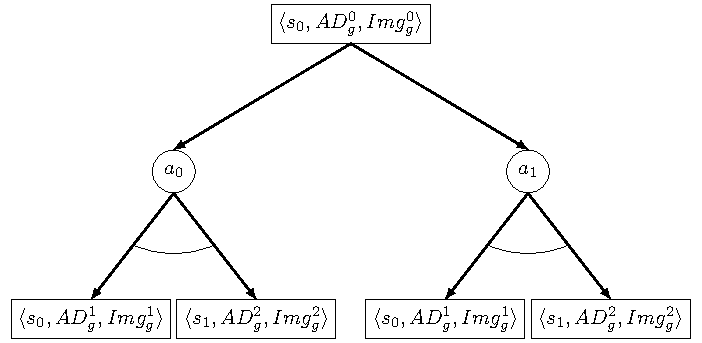
\includegraphics{images/MasterThesisRepNetTreeDraw.pdf}
  \end{center}
  \caption{Look-ahead search space, depth $D=1$ (RepNet-MDP)}\label{fig:repnettree}
\end{figure}

After constructing the search space, an estimation of the value function needs to be back-propagated from the leaves to the root of the tree. An \textit{admissible} heuristic estimate of the true value function
\begin{align}
    h : \Theta_g \rightarrow \R
\end{align}
can be computed at the leaves by taking the base case of the Bellman equations for RepNet-MDPs:
\begin{align}
    h(\theta_g) = \max_{a \in \mathcal{A}} \Big\{ PI_g(s,AD_g,a) \Big\}.
\end{align}
The \textit{epistemic state-action} values are then computed at the action nodes as follows:
\begin{align}
     q(\theta_g, a) = PI_g(s,AD_g,a) + \gamma \sum_{s' \in \mathcal{S}} T_g(g,s,a,s',r_g) h(\big \langle s', \phi_g' \big \rangle).
\end{align}
Non-leaf state nodes use the maximum of the \textit{epistemic state-action} values of their children as their estimate of the value function, i.e.
\begin{align}
    h(\theta_g) = \max_{a \in \mathcal{A}} \Big\{ q(\theta_g, a)  \Big\}.
\end{align}

\section{General discussion: the reputation on a conceptual level}
\label{sec:genn}

The present section briefly discusses the current definition of reputation on a conceptual level and serves as a comment on how it might have to be revised in future work. 

The current definition of reputation (\RefDef{def:repnew}), while arguably intuitive, can lead to undesirable results in regards to self-reputation, fault of its simplicity. This is best demonstrated with an example. Let $A$ and $B$ be two agents, and $Img_A$ agent $A$'s image function, such that:

\begin{align}
    Img_A(B, A) = -1, \,\,\,\,\,\,\,\, Img_A(B,A) = -1,
\end{align}
meaning that in agent $A$'s eyes, $B$ has a poor image of $A$, and $A$ has a poor image of $B$. By definition of the image function, $Img_A(i,i) = 1 \,\,\,\, \forall i \in \mathcal{G}$. As such the self-reputation of agent $A$ is given by:

\begin{align*}
\label{eq:selfrep}
    REP_A(A, Img_A) &= \frac{1}{2} \,\, \big[ Img_A(A,B) \times Img_A(B,A) + Img_A(A,A) \times Img_A(A,A) \big]
    \\&= \frac{1}{2} \,\, \big[ 1 + 1\big] = 1
\end{align*}

Agent $A$ believes its own reputation to be good, despite the fact that it thinks $B$ has a poor image of $A$. Given that $A$ and $B$ are the only agents in the network, this skewed perception of its own reputation could result in agent $A$ performing sub-optimal actions in the network.



\chapter{Testing methodology}
\label{chap:method}

The initial RepNet framework, as described by \textit{Rens et al.} \cite{rensetal}, was developed as a novel extension to the standard POMDP framework, but was subsequently left unimplemented. \RefChap{chap:mdp} covered the simplification process of the RepNet framework to a fully observable setting, in an effort to reduce its intractability. The chapter furthermore discussed an alternative to exact planning such as \textit{value iteration}, called \textit{approximate online} planning, in the context of the simplified RepNet framework. More concretely, a look-ahead search algorithm can be used to approximate the real value function given the current \textit{epistemic state} (\RefSec{sec:onlineplan}). The goal of the present chapter is to present the experimental setup devised to test the framework's properties. \RefSec{sec:testbed} introduces the \textit{scenarios} used to showcase the working principles of the RepNet framework. \RefSec{sec:expset} then details the actual experimental setup. Finally, \RefSec{sec:params} discusses the settings for the parameters that are common across all experiments, while \RefSec{sec:specif} covers the experiment-dependent parameters.

\section{Test bed}
\label{sec:testbed}
This section outlines the \textit{scenarios} that make up the entirety of the experimental setup. Each scenario was designed to showcase specific elements of the RepNet framework. Two types of scenarios are considered in this thesis: \textit{Trading} and \textit{Air-taxi} scenarios. All scenarios are used for different purposes and highlight different aspects of the framework.

\subsection{Trading scenarios}
A \textit{trade transaction} is the activity by which a first party, called the \textit{buyer}, wishes to buy a good from a second party, called the \textit{seller}. A trade transaction materializes when the buyer is willing to buy, and the seller is willing to sell. The trading scenarios used in this thesis involve two to three agents and are designed to showcase the interaction between RepNet and non-RepNet agents.
The first trading scenario, described in \RefEx{ex:trade2ag}, involves two agents and is schematized in \RefFig{fig:ex111}. As the scenario involves only a small number of states, its corresponding transition model is furthermore depicted in \RefFig{fig:ex1}.
\begin{example}[Trade transaction between two agents]
\label{ex:trade2ag}
Let $A$ and $B$ be two agents. Agent $A$ plays the role of the buyer, agent $B$ the role of the seller. Agent $A$ can engage in a trade with agent $B$, and $B$ can accept or refuse the trade offer. Furthermore, agent $A$ can, prior to making a trade offer, do a good deed in an effort to improve its image in the eyes of agent $B$. 
\end{example}
\begin{figure}[h]
    \centering
    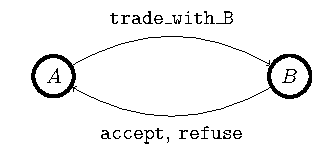
\includegraphics[width=0.35\textwidth]{images/MasterThesisVTOL2agDrawOther.pdf}
    \caption{Trading scenario with two autonomous agents. Agent $A$ can make trade offers, which agent $B$ can accept or refuse.}
    \label{fig:ex111}
\end{figure}
\begin{figure}[h]
    \centering
    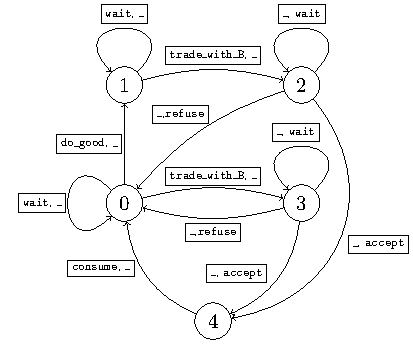
\includegraphics[width=0.75\textwidth]{images/MasterThesisTrade2AgDraw (1).pdf}
    \caption{Transition model of the Trading scenario between agents $A$ and $B$. Node 0 is the starting state, node 1 is the state following agent $A$'s good deed, nodes 2 and 3 are states in which agent $A$ has made an offer and is waiting for $B$'s response, and nodes 4 is the \textit{accept} state.}
    \label{fig:ex1}
\end{figure}



The second trading scenario, described in \RefEx{ex:trade3ag}, involves three agents. The scenario is schematized in \RefFig{fig:ex2}.

\begin{example}[Trading between three agents]
\label{ex:trade3ag}
Let $A$, $B$, and $C$ be three agents. Each agent simultaneously plays the role of buyer and seller, and can thus engage in a trade with any other agent. Each agent can accept or refuse any trade offer made by any remaining agent.
\end{example}
\begin{figure}[h]
  \begin{center}
    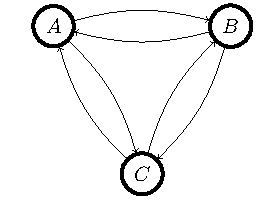
\includegraphics[width=0.31\textwidth]{images/MasterThesistrade3agDraw (3).pdf}
  \end{center}
  \caption{Trading scenario with 3 autonomous agents, each agent can \texttt{trade} with any remaining agent, \texttt{accept}, and \texttt{refuse} trade offers}\label{fig:ex2}
\end{figure}

\subsection{Air-taxi (eVTOL) scenarios}
Electric Vertical Take-off and Landing (eVTOL) aircraft are electric powered aircraft that can can take-off and land vertically, meaning they do not require a runway, and can hover at a given altitude \cite{vtol,vtol56}. Recently, several big companies, including Boeing and NASA, Uber and Lilium GmbH have invested large amounts of money into the development of eVTOL aircraft designed to provide taxi services in and out of cities \cite{vtol2, vtol3}.
These pilotless aircraft make up a network of agents that require air traffic management. Simplified air-taxi scenarios are used in the experimental setup, and are described hereafter.
The first and simplest air-taxi scenario is given in \RefEx{ex:air1} and involves two agents. The scenario is schematized in \RefFig{fig:ex3}.
\begin{example}[Air-taxi battery level management]
\label{ex:air1}
The airspace considered in this example is made up of 1 vertiport, i.e., airport for eVTOL aircraft, as well as a common flying space. The network is made up of 2 eVTOL aircraft, and each aircraft has 3 battery levels (high, medium, low). Upon landing at a vertiport, the battery of an aircraft is fully recharged. A central unit called an oracle, receives the position and battery level of each aircraft at every time-step, and immediately distributes the information to the entire network, thereby bringing the problem to a fully observable setting. At any point in time, only one aircraft may use the vertiport. Each agent's goal is to not run out of battery in the air. The selfish incentive would, therefore, appear to be to stay at the vertiport. This would, however, prevent the other agent from using that same platform, possibly when they most need to. The combined constraint, therefore, lies in the fact that no aircraft may crash at any point in time.
\end{example}

\begin{figure}[h]
  \begin{center}
    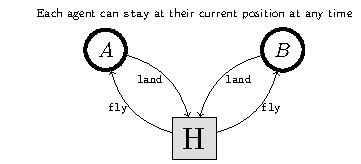
\includegraphics[width=0.5\textwidth]{images/MasterThesisVTOL2agDraw (2).pdf}
  \end{center}
  \caption{Air-taxi scenario with 2 autonomous agents}\label{fig:ex3}
\end{figure}



The second air-taxi scenario, detailed in \RefEx{ex:air2}, involves 4 agents and figures as the most complex example. A scheme of the scenario is given in \RefFig{fig:ex4}.


\begin{example}[Air-taxi travel]
\label{ex:air2}
The airspace considered in this example is designed as a grid that includes 4 vertiports. The network is made up of 4 eVTOL aircraft/agents, each aircraft assumed to have infinite battery. The goal of each agent is to travel to their assigned vertiport along a fixed itinerary, without crashing into any other aircraft. At the start of a run, these agents are randomly placed on the grid somewhere along their axis of travel. Each agent is fully aware of every agent's position on the grid, making the problem fully observable. The selfish goal resides in the fact that each agent wishes to reach their vertiport as quickly as possible. In doing so, the risk of two agents crashing into each other is increased substantially. Agents are, therefore, required to be cooperative, in spite of their selfish intentions \cite{2590}.

\end{example}


\begin{figure}[h]
  \begin{center}
    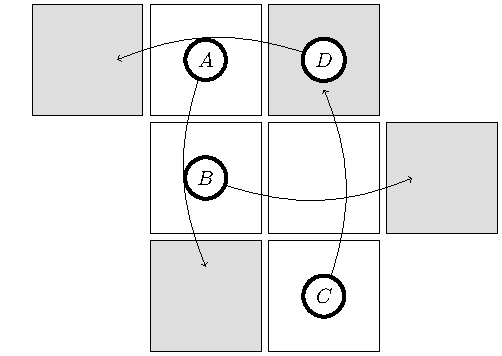
\includegraphics[width=0.48\textwidth]{images/MasterThesisVTOL4Draw (2).pdf}
  \end{center}
  \caption{Air-taxi scenario with 4 autonomous agents}\label{fig:ex4}
\end{figure}


\section{Experimental setup}
\label{sec:expset}
The scenarios described in \RefSec{sec:testbed} are used in a series of experiments designed to test different aspects of the RepNet framework. Concretely, the experimental setup is divided into three parts, which are discussed in the present section. \RefSec{sub:repfeat} deals with tests conducted to test the main properties of the RepNet framework. In \RefSec{sub:adaptrep}, the ability of RepNet agents to quickly adapt to changes in other agents' behavior is discussed. Finally, \RefSec{sub:largescale} extends the experimental setup to include more than two agents.

\subsection{The RepNet framework features}
\label{sub:repfeat}
The first part of the experimental evaluation concerns itself with testing the properties that distinguish RepNet-MDPs from other MDP-derived frameworks, and are thus conducted without the presence of a baseline framework. As a reminder, the properties of the RepNet framework include the notions of \textit{action distribution}, \textit{image}, \textit{reputation}, and \textit{directed actions}. The first series of experiments addresses the first three features, while the second one showcases the benefits and drawbacks of using directed actions. Both series of experiments take part in the environment described in \RefEx{ex:trade2ag}.

\subsubsection{Testing action distribution, image, and reputation}
In this series of experiments, \RefEx{ex:trade2ag} is used as follows: Agent $A$, the \textit{buyer}, is managed by the RepNet algorithm. Agent $B$, the \textit{seller}, is run by a simple algorithm that accepts or rejects trade offers made by agent $A$ according to a set schedule. In particular, agent $B$ is asked to reject trade offers for the 20 first time-steps, accept them for the 60 subsequent time-steps, and finally reject them for the last 20 time-steps. This experiment is averaged over 5 runs consisting of 100 time-steps. The variables tracked are the action distribution, image, and reputation of both agents \textit{in the eyes of the RepNet agent (agent $A$)}. These variables are expected to change with time and, as such, produce tangible changes in the RepNet agent's behavior. The frequency at which agent $A$ makes trade offers is therefore tracked as well.

\subsubsection{Testing directed actions}
\label{sub:directedtest}
The same series of experiments is then coupled with the concept of directed actions, as it was reimagined in \RefSec{sec:reimagined}. In particular, the action of agent $A$ awaiting agent $B$'s response to a trade offer is modeled as a directed action. An important part of using directed actions needs to be addressed here: if the transition probabilities of directed actions depend on the agent's reputation, then a suitable representation of the directed actions' transition model needs to be provided. Said differently, one could easily create a directed transition model that leads agent $A$ to believe that it would be able to engage in a successful trade with agent $B$ regardless of its current reputation. As such, the design of the directed transition model plays an important role in the agent's ability to perform well. Two directed transition models are therefore put to the test, a well-designed model that realistically reflects how the reputation of agent $A$ may influence the willingness of agent $B$ to accept $A$'s trade offers and a poorly designed model with which agent $A$ believes its reputation to have no impact on the outcome of a trade. Both models are schematized in \RefFig{subfig:prof2}. \RefFig{subfig:prof2} furthermore shows the directed transition model equivalent to the situation in which agent $A$ does not make use of directed actions. In fact, if the transition probability of $B$ accepting or refusing the trade offers is equal to $\frac{1}{|\mathcal{A}|}$ (where $|\mathcal{A}|$ is the number of actions at the disposal of agent $B$), regardless of agent $A$'s reputation, then reasoning using directed actions is equivalent to reasoning using undirected actions.




\begin{figure}[h]
\subfloat[Accepting trade offers]
{
\label{subfig:prof2}
\begin{tikzpicture}
\begin{axis}[
    xlabel={$REP_A(A, Img_A)$},
	ylabel= Probability,
	title style={align=left},
	grid=both,
	minor grid style={gray!25},
	major grid style={gray!25},
	legend style={at={(1.0,1.05)},anchor=south east},
	width=0.47\linewidth,
	no marks
    ]
    
    
\addplot+[line width=1pt,solid,color=black] plot coordinates { (0.1, 1/9) (0.3, 1/8) (0.5, 1/7) (0.7, 1/6) (0.9, 1/5)};
\addlegendentry{Well-designed transition model};

\addplot+[line width=1pt,dotted,color=black] plot coordinates { (0.1, 1/3) (0.3, 1/3) (0.5, 1/3) (0.7, 1/3) (0.9, 1/3)};
\addlegendentry{Poorly designed transition model};

\addplot+[line width=1pt,dashed,color=black] plot coordinates { (0.1, 1/6) (0.3, 1/6) (0.5, 1/6) (0.7, 1/6) (0.9, 1/6)};
\addlegendentry{Undirected transition model}; 

\end{axis}
\end{tikzpicture}
}
\quad
\subfloat[Refusing trade offers]
{
\label{subfig:prof4}
\begin{tikzpicture}
\begin{axis}[
    xlabel={$REP_A(A, Img_A)$},
	ylabel= Probability,
	title style={align=left},
	grid=both,
	minor grid style={gray!25},
	major grid style={gray!25},
	legend style={at={(1.0,1.05)},anchor=south east},
	width=0.47\linewidth,
	no marks
    ]
\addplot+[line width=1pt,solid,color=black] plot coordinates { (0.1, 1/5) (0.3, 1/6) (0.5, 1/7) (0.7, 1/8) (0.9, 1/9)};
\addlegendentry{Well-designed transition model};

\addplot+[line width=1pt,dotted,color=black] plot coordinates { (0.1, 1/9) (0.3, 1/9) (0.5, 1/9) (0.7, 1/9) (0.9, 1/9)};
\addlegendentry{Poorly designed transition model};

\addplot+[line width=1pt,dashed,color=black] plot coordinates { (0.1, 1/6) (0.3, 1/6) (0.5, 1/6) (0.7, 1/6) (0.9, 1/6)};
\addlegendentry{Undirected transition model};

\end{axis}
\end{tikzpicture}
}
\caption{Perceived probability of agent $B$ accepting and refusing the trade offers, as a function of the self-reputation of agent $A$.}
\end{figure}




\subsection{Adaptability of the RepNet framework}
\label{sub:adaptrep}


The second part of the experimental evaluation tests the ability of RepNet agents to adapt to changes in the behavior of other agents in the network when adaptation needs to happen quickly. In the previous set of experiments, while agent $B$ had a negative impact on agent $A$ when it refused each trade offer, $A$ could, in theory, turn around the situation, however bad it may be. Said differently, no state in the transition model represented a \textit{trap} that is impossible to escape. 
In \RefEx{ex:air1}, the scenario used in this section, if one agent starts monopolizing the vertiport for more time-steps than are necessary, the other agent is expected to quickly change its strategy in a way that minimizes the chances of crashes occurring. Failing to do so could result in the second agent not being able to land when absolutely necessary. From an implementational point of view, a crash is represented as a \textit{trap} state, and is, therefore, to be avoided at all costs.


To test the adaptability of RepNet agents, agent $A$ is managed by the RepNet algorithm, while agent $B$ is controlled by a simple algorithm that gradually increases the average time it spends on the vertiport. Agent $A$ is expected to be able to pick up on these changes and adapt its own behavior accordingly.
Specifically, agents $A$ and $B$ both start in the airspace, with their batteries fully charged. Agent $B$ is designed to initially only make use of the vertiport when absolutely necessary, i.e., when its battery is low. Every $10$ time-steps, Agent $B$'s selfishness is increased by a fixed factor $\xi \in [0,1]$. Concretely, $\xi$ represents the probability of agent $B$ deciding to stay at the vertiport for the following time-step. As the battery is fully recharged immediately upon landing at the vertiport, deciding to stay on the ground is perceived as a selfish and unnecessary move by agent $B$. 
2 series of 15 consecutive runs of 50 time-steps are conducted as follows:
\begin{itemize}
    \item The first series of runs aims at tracking the number of crashes that occur as a function of the number of time-steps. As the selfishness of agent $B$ increases, the likelihood of a crash does so as well.
    \item In the second series of experiments, agent $B$'s behavior is altered slightly: it will never choose to remain on the ground when agent $A$'s battery is low. This change makes it possible to uninterruptedly observe the behavioral changes of the RepNet agents across the 50 time-steps.
\end{itemize}
In an effort to provide an idea of how robust to changes in the behavior of agent $B$ the RepNet agent is, the same experiment is conducted under the same circumstances with agent $A$ now controlled by a standard \textit{MDP look-ahead} algorithm (\RefSec{sec:stateart}). Standard MDP-based algorithms are, by definition, incapable of adapting to behavioral changes of other agents, as these changes would have to be reflected in updates to the transition model. This MDP-based algorithm, therefore, serves as a baseline for comparison in this experiment.

As the \textit{immediate reward function} $\mathcal{R}$ of MDP agents is different from the \textit{perceived immediate impact} $PI$ of RepNet agents, the reward function was defined to be equal to the initial perceived impact of the RepNet agent, i.e.:
\begin{align}
    \forall s \in \mathcal{S}, \forall a \in \mathcal{A}: \mathcal{R}(s,a) = PI_g(s, AD_g^0, a)
\end{align}
where $AD_g^0(h,s)(a) = \frac{1}{|\mathcal{A}|} \,\, \forall h \in \mathcal{G}, \forall s \in \mathcal{S}, \forall a \in \mathcal{A}$. 



%The same experiment is furthermore conducted with the model-free learning algorithm called Q-Learning, using the $\epsilon$-greedy \textit{exploration-exploitation} strategy. The Q-Learning algorithm, although not designed to be used in dynamic environments, is, due to its ability to implicitly learn the transition through experience, expected to be robust \textit{to some degree} to gradual changes in the environment dynamics. \textcolor{red}{Not present yet}

The RepNet agent is expected to be able to sacrifice its selfish intentions, which would be to use the vertiport when in the air and leave the vertiport after landing, in an effort to avoid crashes.


\subsection{Large-scale experiments}
\label{sub:largeexp}
In the final part of the experimental evaluation, the ability of the RepNet algorithm to deal with an increased number of selfish agents is tested. To this end, Examples \ref{ex:trade3ag} and \ref{ex:air2} from the test bed are used hereafter. 

\subsubsection{Large-scale trading experiment}
\RefEx{ex:trade3ag} is used to verify the ability of a RepNet agent, say agent $A$, to manage its trades with the two remaining agents $B$ and $C$ (control agents), based not only on their behavior towards the agent of interest but also their behavior with each other. In fact, the action distribution, image, and reputation are general constructs, that is, they are not limited to tracking interactions that impact the RepNet agent \textit{directly}. 

The experiment can be divided into three parts: in the first part, agent $B$ is asked to refuse each trade offer made by agent $A$, while agent $C$ is expected to accept each trade offer coming from that same agent. This portion of the experiments assesses the ability of the RepNet agent (agent $A$) to accurately determine which agent it is more likely to successfully engage in trades with. In the second part, the roles are switched, and agent $B$ accepts the trade offers, while agent $C$ refuses them. This portion assesses the ability of the agent of interest to \textit{unlearn} what it has learned and adapt its behavior accordingly. 
In the third and final part, the RepNet agent's actions are \textit{blocked} from having any effect on the environment, preventing said agent from accumulating knowledge based on communications it is directly affected by. Furthermore, agents $B$ and $C$ are asked to engage in trades with each other. Agent $B$ is asked to reject all trade offers, while agent $C$ is asked to accept all trade offers. This portion of the experiment aims at testing the ability of the RepNet agent to draw conclusions on how it should act based on interactions it is not directly affected by. In fact, while the RepNet agent's actions have no effect on the environment, they are still recorded in this experiment and provide insight into which agent it is more likely to trade with. As the results described in \RefChap{chap:res} will show, Agent $A$ is, in fact, unable to adapt its behavior in these instances.


\subsubsection{Large-scale air-taxi experiment}
A final experiment is conducted using \RefEx{ex:air2} as the testing ground. The goal of this experiment is to demonstrate the ability of multiple RepNet agents to learn to cooperate with one another, despite their selfish intentions \cite{2590}. This experiment ties into the notion of \textit{convergence} in \textit{Multi-agent learning} (MAL), which was briefly discussed in \RefSec{sec:additional}. In particular, three of the four agents are controlled by their respective instances of the RepNet algorithm, while the last agent is controlled by a \textit{control} algorithm. Concretely, the control agent is initially tuned to be entirely selfless, i.e., it will always prioritize the other agents reaching their destination \textit{first} over reaching its own vertiport itself. Every $20$ time-steps, the selfishness of the fourth agent is gradually increased by a constant factor $\xi \in [0,1]$. $\xi$ represents the probability with which the control agent decides to move forward in situations in which the selfless move would be to stay in place. The RepNet agents are expected to notice these behavioral changes and adapt their own behavior accordingly. In doing so, they, however, alert the remaining RepNet agents of their own behavior change, forcing them to take these changes into account as well. 
The experiment itself runs for 100 time-steps. The agents are initially randomly dropped in the environment somewhere along their axis of travel. Each time every agent reaches its designated vertiport, the successful run is recorded, and the agents are randomly placed back in the environment. Each time a crash occurs, the unsuccessful run is recorded, and the agents are likewise randomly placed back in the environment. 


\label{sub:largescale}
\section{General parameters}
\label{sec:params}

\subsection{RepNet parameters}

\subsubsection{The image update function $\mathcal{U}$}
\label{sub:updatenn}

Given a current image value $v = Img_A(B,C)$ describing the image $C$ has of $B$, according to $A$, a learning rate $\alpha$, and the expected impact $i = ETI_A(B,C,s,AD_A)$ that $C$ has on $B$ when performing one of its actions in current the state $s$, $\mathcal{U}(\alpha, v, i)$ (\RefDef{def:systempo}) returns the updated value $v' = Img_A'(B,C)$. Agent $A$'s behavior is dictated by the image it believes each agent in the network to have of each other. Consequently, the image update function $\mathcal{U}$ has an important impact on $A$'s performance.
Two instantiations of the update function $\mathcal{U}$ are proposed by \textit{Rens et al.} \cite{rensetal}, namely the \textit{difference} update and the \textit{saturation} update.  

\begin{itemize}
    \item Difference update: 
    \begin{align}
    \mathcal{U}(\alpha, v, i) :=
        \begin{dcases}
            v + \alpha (1-v)i &\text{ if } i \geq 0
            \\
            v + \alpha (1+v)i &\text{ if } i < 0
        \end{dcases}
    \end{align}
    
    \item Saturation update: 
    \begin{align}
    \mathcal{U}(\alpha, v, i) :=
        \begin{dcases}
            1 &\text{ if } v + \alpha i > 1
            \\
            -1 &\text{ if } v + \alpha i < -1
            \\
            v + \alpha i &\text{ otherwise }
        \end{dcases}
    \end{align}
\end{itemize}

The update surfaces are shown in \RefFig{fig:upd} for $\alpha = 0.5$. The experiments discussed in this chapter were all conducted using the difference update, as it produced the most consistent results across all experiments. Note that this does not mean that the saturation update is of inferior quality. In fact, a small portion of the experiments was indeed found to work better with the saturation update, which is indicative of the domain-dependence of the \textit{image update function}. Nevertheless, in an attempt to keep the results consistent between tests, in particular those that make use of the same test bed, the same function was kept throughout the experimental evaluation.


\begin{figure}[h]
\subfloat[Difference update]
{
\label{subfig:update1}
    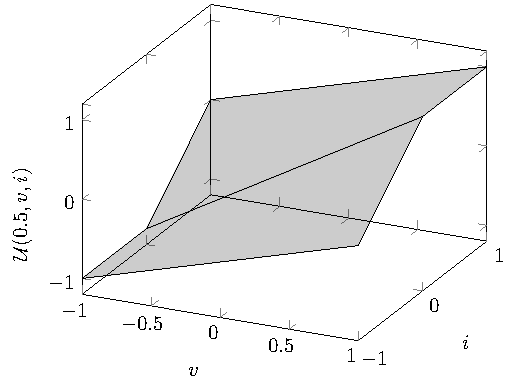
\includegraphics[width=0.48\textwidth]{images/MasterThesisUpdateDraw2.pdf}
}
\subfloat[Saturation update]
{
\label{subfig:update2}
    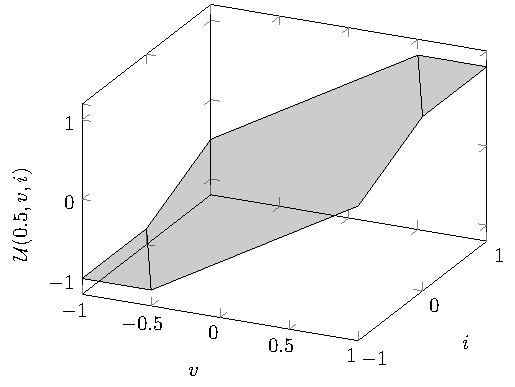
\includegraphics[width=0.48\textwidth]{images/MasterThesisUpdateDraw3.pdf}
}
\caption{Image update functions proposed by \textit{Rens et al.} \cite{rensetal}. The learning rate $\alpha$ is set to 0.5}
\label{fig:upd}
\end{figure}

\subsubsection{Expected total impact trade-off parameter $\delta$}
The trade-off parameter $\delta \in [0,1]$ in the expected total impact between agents $h$ and $i$ according to $g$, written $ETI(h,i,s,AD_g)$, trades off the relative importance of the impact due to agent $h$ and the impact perceived by $h$ (\RefDef{def:imp}). This parameter was set to $0.8$ across all experiments, that is, whenever $g$'s opinion on the image that $i$ has of $h$ ($Img_g(h,i)$) is updated, more weight will be given to the expected impact that $i$ has on $h$ in the current state, as opposed to the expected impact that $h$ has on $i$. Said differently, the image that a first agent $i$ has of another agent $h$ is conditioned mainly by $i$'s likeliness to impact (positively or negatively) $h$ in the current state $s$.

\subsubsection{Discount factor $\gamma$}
The discount factor $\gamma \in [0,1]$ in the RepNet framework's value function (\RefDef{def:opti}) determines the importance future time-steps should have on the agent's decision-making process. The closer it is to 1, the more important the future is, the closer it is to 0, the more important the present is. The value was set to 0.7 across all experiments.

\subsubsection{Initial settings for the action distribution and the image}
The RepNet agents deployed in a new environment are assumed to have no preconceived notions of other agents' behavior, reputation, and image of one another. This translates to the following initial settings for the action distribution and image for agent $g$:
\begin{align}
\begin{split}
    AD_g^0(h,s)(a) = \frac{1}{|\mathcal{A}|} \,\,\,\, \forall h \in \mathcal{G}, \forall s \in \mathcal{S}, &\forall a \in \mathcal{A},
    \\Img_g(h,i) = 0 \,\,\,\, \forall h, i \in \mathcal{G}, h \neq &i.
\end{split}
\end{align}

\subsection{MDP parameters}
\subsubsection{Discount factor $\gamma$}
The discount factor $\gamma \in [0,1]$ in the MDP framework's value function plays the same role as in the RepNet framework and was likewise set to 0.7 across all experiments involving an MDP agent.

\subsubsection{Look-ahead depth $D$}
The scenarios in which an MDP agent is used feature a look-ahead depth $D = 3$, as the same depth is used for the RepNet agents in said scenarios.


\section{Experiment-specific parameters}
\label{sec:specif}
Several parameters were tailored to each experiment separately. This section aims at summarizing the settings for these parameters. 

As such, $D$ is defined as the look-ahead depth of the online search algorithm used by RepNet agents (\RefSec{sec:onlineplan}). The higher it is, the more informed the RepNet agent's decisions can be. This comes at the drawback of increased computation times. \RefSec{sub:updatenn} reviewed the concept of image update function. This function takes a parameter $\alpha \in [0,1]$ called the learning rate that determines how quickly the image function is updated. $\eta$ is the \textit{Laplace} smoothing parameter and was introduced in \RefSec{sec:reduct} in an effort to smooth out the action distribution, especially in cases where the transition models are deterministic.

The only parameter that has not been discussed thus far is the \textit{exploration-exploitation trade-off parameter} $\epsilon$. In order for the RepNet agent to learn, sometimes it must be forced to try out actions even if the associated value is significantly lower than that of another action. In fact, in the trading examples between agents $A$ and $B$, if $A$ realizes $B$'s unwillingness to accept the trade offers, the value associated with the \texttt{trade\_with\_B} action decreases. If now $B$ changes its strategy and accepts all trade offers, $A$ can not know of this change unless it attempts to trade with $B$ occasionally. This concept is known in the literature as the \textit{exploration-exploitation trade-off} \cite{cassano2019isl}. \textit{Exploration} refers to the phase in which an agent performs actions that it would otherwise consider to be sub-optimal. \textit{Exploitation} refers to the phase in which an agent utilizes its current policy to move about in the environment. Several strategies for balancing \textit{exploration} and \textit{exploitation} exist, some simpler, others more complex. As the primary goal of this thesis does not lie in evaluating the benefits and drawbacks of different strategies, the arguably simplest strategy, called $\epsilon$-greedy, was used \cite{epsi}. The $\epsilon$-greedy strategy consists in selecting a random action $a \in \mathcal{A}$ at each time-step with a fixed probability $\epsilon \in [0,1]$, instead of selecting the action $a^\star$ that would, given the current policy, be considered optimal. The $\epsilon$-greedy strategy was solely utilized in the trading experiments, as using it with the air-taxi experiments can easily lead to crashes, and thus tarnish the significance of the results.
The settings for each parameter and experiment are summarized in Table \ref{tab:t1}.
\begin{table*}[h]
\centering
\begin{tabular}{c c c c c}
    \toprule
    \midrule
    \multirow{2}[4]{*}{Trading between 2 agents} & \multicolumn{4}{c}{Parameters}\\ 
    \cmidrule(rl){2-5}
    & $D$  & $\epsilon$ & $\alpha$ & $\eta$ \\ 
    \cmidrule(r){1-1}\cmidrule(l){2-5}
    \multicolumn{1}{l}{RepNet agent $A$}& 3 & 0.2 & 0.8 & 0.1   \\
    \midrule
    
    \multirow{2}[4]{*}{Trading between 3 agents} & \multicolumn{4}{c}{Parameters}\\ 
    \cmidrule(rl){2-5}
    & $D$  & $\epsilon$ & $\alpha$ & $\eta$  \\ 
    \cmidrule(r){1-1}\cmidrule(l){2-5}
    \multicolumn{1}{l}{RepNet agent $A$}& 3 & 0.2 & 0.8 & 0.1   \\
    \midrule
    
    \multirow{2}[4]{*}{Air-taxi with 2 agents} & \multicolumn{4}{c}{Parameters}\\ 
    \cmidrule(rl){2-5}
    & $D$  & $\epsilon$ & $\alpha$ & $\eta$  \\ 
    \cmidrule(r){1-1}\cmidrule(l){2-5}
    \multicolumn{1}{l}{RepNet agent $A$}& 3 & 0 & 1 & 0.15   \\
    \midrule
    
    \multirow{2}[4]{*}{Air-taxi with 4 agents} & \multicolumn{4}{c}{Parameters}\\ 
    \cmidrule(rl){2-5}
    & $D$  & $\epsilon$ & $\alpha$ & $\eta$   \\ 
    \cmidrule(r){1-1}\cmidrule(l){2-5}
    \multicolumn{1}{l}{RepNet agent $A$}& 2 & 0 & 1 & 0.1   \\
    \multicolumn{1}{l}{RepNet agent $B$}& 2 & 0 & 1 & 0.1   \\
    \multicolumn{1}{l}{RepNet agent $C$}& 2 & 0 & 1 & 0.1   \\
    \midrule
    \bottomrule
\end{tabular}
        %\centering
\caption{Settings for the experiment-specific parameters, for each of the experiments.}
\label{tab:t1}
\end{table*}


\chapter{Results}
\label{chap:res}

This chapter covers the findings of the experiments described in \RefChap{chap:method}. These experiments aim at quantifying the performance of the RepNet algorithm in both simple and more complex scenarios while demonstrating its strong points, as well as shortcomings. 
The chapter follows the following structure: in \RefSec{sec:feat}, the fundamental properties that differentiate the RepNet framework from other MDP-derived frameworks are presented. \RefSec{sec:adapt} covers the ability of the algorithm to quickly adapt to changes in the behavior of other agents. \RefSec{sec:large} presents the results related to the two large-scale experiments. Finally, \RefSec{sec:summa} summarizes the results.

\section{The properties of the RepNet framework}
\label{sec:feat}
In this section, the concepts of \textit{action distribution}, \textit{image}, \textit{reputation}, and \textit{directed actions}, as well as these concepts' effects on RepNet agents' behavior, are quantified. The results of two sets of experiments are presented hereafter. The first set of experiments covers  \textit{action distribution}, \textit{image}, \textit{reputation} in the absence of \textit{directed actions}, while the second set covers the same properties in their presence.

\subsection{Testing action distribution, image, and reputation}
The \textit{action distribution}, \textit{image}, and \textit{reputation} of agent $A$ are tracked throughout the experiment, which is made up of 5 runs, of which the average one is analyzed hereafter. As such, \RefFig{subfig:paccept} shows the evolution of agent $A$'s action distribution for target agent $B$ in state $s = 2$ (the state in which $B$ is aware of the trade offer made by agent $A$, which has done a good deed prior to the offer, see \RefFig{fig:ex1}). \RefFig{subfig:image} displays the image $B$ has of $A$ and vice versa, according to $A$.
\RefFig{subfig:rep} shows the reputation of $A$ and $B$, according to $A$. Finally, \RefFig{subfig:freq} displays the tangible effects of these variables on $A$'s behavior. Concretely it shows the evolution of the frequency at which $A$ makes trade offers. Note that to maintain clarity, a shorthand notation for the reputation is used in this chapter, that is,
\begin{align}
    REP_g(h,Img_g) = REP_g(h) \,\,\,   \forall g, h \in \mathcal{G}.
\end{align}

In the first 20 time-steps, $B$ refuses each trade offer. Agent $A$ is able to pick up on this via the action distribution. As a consequence, it quickly reduces the frequency at which it attempts to trade with $B$. $A$'s image of $B$, and, by extension, $B$'s reputation (\RefDef{def:repnew}) quickly drop alongside. Interestingly, $A$'s self-reputation decreases in a similar fashion. In fact, $B$ refusing to trade with $A$ can be explained as having two effects on $A$'s perception of the network, both following from the current mathematical definition of reputation (\RefDef{def:repnew}):
\begin{itemize}
    \item $B$ is an unreliable agent and should, therefore, have a poor reputation. The image $A$ has of $B$ decreases, and consequently, so does $B$'s reputation.
    \item $B$ refuses to trade with $A$ because it believes $A$ to be unreliable. $A$ must adapt its self-reputation based on the evidence it is provided with. In this case, the evidence points towards the fact that $A$ might be seen as unreliable in the network, which only includes $B$. 
\end{itemize}
The similarity between $A$'s and $B$'s reputations can be further explained by the fact that the network is made up of only two agents. As such, the evidence provided to $A$ is insufficient for it to make up its mind as to the cause of $B$'s changes in behavior.



In the 60 following time-steps, $B$ is asked to change its behavior and accept each trade offer. Hesitant at first, $A$ gradually increases the frequency at which it attempts to trade with $B$. $B$'s reputation, as well as $A$'s self-reputation, are positively impacted by $B$'s change of behavior. The same two-effect explanation can be applied to explain the increase of both agents' reputations.

Finally, $B$ reverts back to its old behavior during the final 20 steps. Again, Agent $A$ is able to pick up on this change and adapt its behavior accordingly.

\begin{figure}[h]
\subfloat[Probability of $B$ accepting and refusing $A$'s trade offers, according to $A$]
{
\label{subfig:paccept}
\begin{tikzpicture}
\begin{axis}[
	xlabel=Time-steps,
	ylabel= Probability,
	title style={align=left},
	grid=both,
	minor grid style={gray!25},
	major grid style={gray!25},
	legend style={at={(1.0,1.05)},anchor=south east},
	width=0.47\linewidth,
	no marks]
\addplot[line width=1pt,solid,color=black] %
	table[x=b,y=a,col sep=comma]{CSV/tradeABaccept2u.csv};
\addlegendentry{$AD_A(B,2)(\texttt{accept})$};

\addplot[line width=1pt,dotted,color=black] %
	table[x=b,y=a,col sep=comma]{CSV/tradeABrefuse2u.csv};
\addlegendentry{$AD_A(B,2)(\texttt{refuse})$};


\draw [densely dashed, line width=1.5pt] (20,0) -- (20,1);
\draw [densely dashed, line width=1.5pt] (80,0) -- (80,1);

\end{axis}
\end{tikzpicture}
}
\quad
\subfloat[Image agents $A$ and $B$ have of each other, according to $A$]
{
\label{subfig:image}
\begin{tikzpicture}
\begin{axis}[
	xlabel=Time-steps,
	ylabel= Image,
	title style={align=left},
	grid=both,
	minor grid style={gray!25},
	major grid style={gray!25},
	legend style={at={(1.0,1.05)},anchor=south east},
	width=0.47\linewidth,
	no marks]
\addplot[line width=1pt,solid,color=black] %
	table[x=b,y=a,col sep=comma]{CSV/tradeABimgABu.csv};
\addlegendentry{$Img_A(B,A)$};

\addplot[line width=1pt,dotted,color=black] %
	table[x=b,y=a,col sep=comma]{CSV/tradeABimgBAu.csv};
\addlegendentry{$Img_A(A,B)$};

\draw [densely dashed, line width=1.5pt] (20,-2) -- (20,2);
\draw [densely dashed, line width=1.5pt] (80,-2) -- (80,2);
\end{axis}
\end{tikzpicture}
}
\caption{Undirected actions: Evolution of the action distribution and image function, according to agent $A$.}
\end{figure}

\begin{figure}[h]
\subfloat[Reputation of agents $A$ and $B$, according to $A$]
{
\label{subfig:rep}
\begin{tikzpicture}
\begin{axis}[
	xlabel=Time-steps,
	ylabel= Reputation,
	title style={align=left},
	grid=both,
	minor grid style={gray!25},
	major grid style={gray!25},
	legend style={at={(0.98,0.02)},anchor=south east},
	width=0.465\linewidth,
	no marks]
\addplot[line width=1pt,solid,color=black] %
	table[x=b,y=a,col sep=comma]{CSV/tradeABrepAu.csv};
\addlegendentry{$REP_A(A)$};

\addplot[line width=1pt,dotted,color=black] %
	table[x=b,y=a,col sep=comma]{CSV/tradeABrepBu.csv};
\addlegendentry{$REP_A(B)$};

\draw [densely dashed, line width=1.5pt] (20,-2) -- (20,2);
\draw [densely dashed, line width=1.5pt] (80,-2) -- (80,2);
\end{axis}
\end{tikzpicture}
}
\quad
\subfloat[Frequency of the trade offers made by $A$, measured in 5 time-step intervals]
{
\label{subfig:freq}
\begin{tikzpicture}
\begin{axis}[
    xlabel=Time-steps,
	ylabel= Frequency,
	title style={align=left},
	grid=both,
	minor grid style={gray!25},
	major grid style={gray!25},
	legend style={at={(1.0,1.05)},anchor=south east},
	width=0.465\linewidth,
	no marks
    ]
\addplot+[line width=1pt,solid,color=black] plot coordinates { (0, 1.6) (5, 1.4) (10, 1) (15, 0.4) (20, 0.2) (25, 0.4)(30, 0.4)(35, 0.4)(40, 0.8)(45, 0.6)(50, 0.8)(55, 0.6)(60, 0.6)(65, 0.6)(70, 0.8)(75, 1)(80, 0.8)(85, 1)(90, 0.8)(95, 0.2)};

\draw [densely dashed, line width=1.5pt] (20,-2) -- (20,2);
\draw [densely dashed, line width=1.5pt] (80,-2) -- (80,2);
\end{axis}
\end{tikzpicture}
}
\caption{Undirected actions: Evolution of the reputation according to agent $A$, and frequency of trade offers made by agent $A$.}
\end{figure}




\subsection{Testing directed actions}

The same set of experiments was conducted again, now using the concept of \textit{directed actions}. As discussed in \RefSec{sub:directedtest}, the design of the directed transition model has a significant impact on the performance of the RepNet agent. Two directed transition models of vastly different quality were proposed, and the results are described hereafter.

\subsubsection{Well-designed directed transition model}

Analogously to the previous section, \RefFig{subfig:paccept2} shows the evolution of agent $A$'s action distribution for agent $B$ in state $s = 2$, \RefFig{subfig:image2} displays the image $B$ has of $A$ and vice versa, \RefFig{subfig:rep2} shows the reputation of $A$ and $B$, and \RefFig{subfig:freq2} displays the tangible effects of these variables on $A$'s behavior. 

The well-designed transition model noticeably improves the performance of the RepNet agent. While the trajectories showcase the same key elements as in the previous section, the pace at which agent $A$ is able to adapt has greatly improved. As $B$ refuses the offers during the 20 first time-steps, its reputation decreases along with $A$'s self-reputation. The directed transition model was designed such that agent $A$ believes that its reputation must be good for $B$ to be willing to trade with $A$ (\RefFig{subfig:prof2} and \RefFig{subfig:prof4}). As such, $A$'s relatively poor-in-comparison self-reputation has an immediate effect on the \textit{value} it associates with action \texttt{trade\_with\_B} during the look-ahead search. Said differently, it quickly becomes more \textit{valuable} to pick a different action over \texttt{trade\_with\_B}. This explains the rash changes in $A$'s behavior at the start. Incidentally, agent $A$ is able to quickly increase the rate at which it attempts to trade with $B$ once it notices $B$'s willingness to trade. The average rate ends up topping off higher than without the use of directed transitions.

\begin{figure}[h]
\subfloat[Probability of $B$ accepting and refusing $A$'s trade offers, according to $A$]
{
\label{subfig:paccept2}
\begin{tikzpicture}
\begin{axis}[
	xlabel=Time-steps,
	ylabel= Probability,
	title style={align=left},
	grid=both,
	minor grid style={gray!25},
	major grid style={gray!25},
	legend style={at={(1.0,1.05)},anchor=south east},
	width=0.47\linewidth,
	no marks]
\addplot[line width=1pt,solid,color=black] %
	table[x=b,y=a,col sep=comma]{CSV/tradeABaccept2.csv};
\addlegendentry{$AD_A(B,2)(\texttt{accept})$};

\addplot[line width=1pt,dotted,color=black] %
	table[x=b,y=a,col sep=comma]{CSV/tradeABrefuse2.csv};
\addlegendentry{$AD_A(B,2)(\texttt{refuse})$};

\draw [densely dashed, line width=1.5pt] (20,-2) -- (20,2);
\draw [densely dashed, line width=1.5pt] (80,-2) -- (80,2);
\end{axis}
\end{tikzpicture}
}
\quad
\subfloat[Image agents $A$ and $B$ have of each other, according to $A$]
{
\label{subfig:image2}
\begin{tikzpicture}
\begin{axis}[
	xlabel=Time-steps,
	ylabel= Image,
	title style={align=left},
	grid=both,
	minor grid style={gray!25},
	major grid style={gray!25},
	legend style={at={(1.0,1.05)},anchor=south east},
	width=0.47\linewidth,
	no marks]
\addplot[line width=1pt,solid,color=black] %
	table[x=b,y=a,col sep=comma]{CSV/tradeABimgAB.csv};
\addlegendentry{$Img_A(B,A)$};

\addplot[line width=1pt,dotted,color=black] %
	table[x=b,y=a,col sep=comma]{CSV/tradeABimgBA.csv};
\addlegendentry{$Img_A(A,B)$};

\draw [densely dashed, line width=1.5pt] (20,-2) -- (20,2);
\draw [densely dashed, line width=1.5pt] (80,-2) -- (80,2);
\end{axis}
\end{tikzpicture}
}
\caption{Well-designed directed transition model: Evolution of the action distribution and image function, according to agent $A$.}
\end{figure}

\begin{figure}[h]
\subfloat[Reputation of agents $A$ and $B$, according to $A$]
{
\label{subfig:rep2}
\begin{tikzpicture}
\begin{axis}[
	xlabel=Time-steps,
	ylabel= Reputation,
	title style={align=left},
	grid=both,
	minor grid style={gray!25},
	major grid style={gray!25},
	legend style={at={(0.57,0.70)},anchor=south east},
	width=0.465\linewidth,
	no marks]
\addplot[line width=1pt,solid,color=black] %
	table[x=b,y=a,col sep=comma]{CSV/tradeABrepA.csv};
\addlegendentry{$REP_A(A)$};

\addplot[line width=1pt,dotted,color=black] %
	table[x=b,y=a,col sep=comma]{CSV/tradeABrepB.csv};
\addlegendentry{$REP_A(B)$};

\draw [densely dashed, line width=1.5pt] (20,-2) -- (20,2);
\draw [densely dashed, line width=1.5pt] (80,-2) -- (80,2);
\end{axis}
\end{tikzpicture}
}
\quad
\subfloat[Frequency of the trade offers made by $A$, measured in 5 time-step intervals]
{
\label{subfig:freq2}
\begin{tikzpicture}
\begin{axis}[
    xlabel=Time-steps,
	ylabel= Frequency,
	title style={align=left},
	grid=both,
	minor grid style={gray!25},
	major grid style={gray!25},
	legend style={at={(1.0,1.05)},anchor=south east},
	width=0.465\linewidth,
	no marks
    ]
\addplot+[line width=1pt,solid,color=black] plot coordinates { (0, 1.4) (5, 0.6) (10, 0.4) (15, 0) (20, 0) (25, 0)(30, 0)(35, 0)(40, 0)(45, 0.8)(50, 0.6)(55, 0.6)(60, 0.8)(65, 1)(70, 0.8)(75, 1.4)(80, 1)(85, 1)(90, 0.4)(95, 0)};

\draw [densely dashed, line width=1.5pt] (20,-2) -- (20,2);
\draw [densely dashed, line width=1.5pt] (80,-2) -- (80,2);
\end{axis}
\end{tikzpicture}
}
\caption{Well-designed directed transition model: Evolution of the reputation according to agent $A$, and frequency of trade offers made by agent $A$.}
\end{figure}





\subsubsection{Poorly designed directed transition model}
The same set of experiments was conducted a third time with a poorly designed \textit{directed transition model}. As discussed in \RefSec{sub:directedtest}, the presently used directed transition model aims at making agent $A$ believe that agent $B$ will want to trade with $A$ in spite of a poor reputation. \RefFig{subfig:paccept3} displays the evolution of agent $A$'s action distribution for agent $B$, \RefFig{subfig:image3} shows the image $B$ has of $A$ and vice versa, \RefFig{subfig:rep3} shows the reputation of $A$ and $B$, and \RefFig{subfig:freq3} displays the tangible effects of these variables on $A$'s behavior.

The present experiment demonstrates that the presence of directed actions does not guarantee that the RepNet agent will perform better. In fact, a poorly designed directed transition model mitigates many of the benefits initially obtained by introducing the concepts of \textit{action distribution}, \textit{image}, and \textit{reputation}. In fact, the \textit{action distribution}, \textit{image}, and \textit{reputation} trajectories show that although the algorithm is capable of noticing the same changes in $B$'s behavior, the fact that it believes its reputation to be of little importance prevents it from adapting its own behavior. Consequently, agent $A$ has become slow at learning from other agents' behavior.
\begin{figure}[h]
\subfloat[Probability of $B$ accepting and refusing $A$'s trade offers, according to $A$]
{
\label{subfig:paccept3}
\begin{tikzpicture}
\begin{axis}[
	xlabel=Time-steps,
	ylabel= Probability,
	title style={align=left},
	grid=both,
	minor grid style={gray!25},
	major grid style={gray!25},
	legend style={at={(1.0,1.05)},anchor=south east},
	width=0.465\linewidth,
	no marks]
\addplot[line width=1pt,solid,color=black] %
	table[x=b,y=a,col sep=comma]{CSV/tradeABaccept2b.csv};
\addlegendentry{$AD_A(B,2)(\texttt{accept})$};

\addplot[line width=1pt,dotted,color=black] %
	table[x=b,y=a,col sep=comma]{CSV/tradeABrefuse2b.csv};
\addlegendentry{$AD_A(B,2)(\texttt{refuse})$};

\draw [densely dashed, line width=1.5pt] (20,-2) -- (20,2);
\draw [densely dashed, line width=1.5pt] (80,-2) -- (80,2);
\end{axis}
\end{tikzpicture}
}
\quad
\subfloat[Image agents $A$ and $B$ have of each other, according to $A$]
{
\label{subfig:image3}
\begin{tikzpicture}
\begin{axis}[
	xlabel=Time-steps,
	ylabel= Image,
	title style={align=left},
	grid=both,
	minor grid style={gray!25},
	major grid style={gray!25},
	legend style={at={(1.0,1.05)},anchor=south east},
	width=0.465\linewidth,
	no marks]
\addplot[line width=1pt,solid,color=black] %
	table[x=b,y=a,col sep=comma]{CSV/tradeABimgABb.csv};
\addlegendentry{$Img_A(B,A)$};

\addplot[line width=1pt,dotted,color=black] %
	table[x=b,y=a,col sep=comma]{CSV/tradeABimgBAb.csv};
\addlegendentry{$Img_A(A,B)$};

\draw [densely dashed, line width=1.5pt] (20,-2) -- (20,2);
\draw [densely dashed, line width=1.5pt] (80,-2) -- (80,2);
\end{axis}
\end{tikzpicture}
}
\caption{Poorly designed directed transition model: Evolution of the action distribution and image function, according to agent $A$.}
\end{figure}


\begin{figure}[h]
\subfloat[Reputation of agents $A$ and $B$, according to $A$]
{
\label{subfig:rep3}
\begin{tikzpicture}
\begin{axis}[
	xlabel=Time-steps,
	ylabel= Reputation,
	title style={align=left},
	grid=both,
	minor grid style={gray!25},
	major grid style={gray!25},
	legend style={at={(0.87,0.02)},anchor=south east},
	width=0.47\linewidth,
	no marks]
\addplot[line width=1pt,solid,color=black] %
	table[x=b,y=a,col sep=comma]{CSV/tradeABrepAb.csv};
\addlegendentry{$REP_A(A)$};

\addplot[line width=1pt,dotted,color=black] %
	table[x=b,y=a,col sep=comma]{CSV/tradeABrepBb.csv};
\addlegendentry{$REP_A(B)$};

\draw [densely dashed, line width=1.5pt] (20,-2) -- (20,2);
\draw [densely dashed, line width=1.5pt] (80,-2) -- (80,2);
\end{axis}
\end{tikzpicture}
}
\quad
\subfloat[Frequency of the trade offers made by $A$, measured in 5 time-step intervals]
{
\label{subfig:freq3}
\begin{tikzpicture}
\begin{axis}[
    xlabel=Time-steps,
	ylabel= Frequency,
	title style={align=left},
	grid=both,
	minor grid style={gray!25},
	major grid style={gray!25},
	legend style={at={(1.0,1.05)},anchor=south east},
	width=0.47\linewidth,
	no marks
    ]
\addplot+[line width=1pt,solid,color=black] plot coordinates { (0, 1.8) (5, 1.2) (10, 1.8) (15, 1.6) (20, 1.2) (25, 1.2)(30, 0.8)(35, 1.2)(40, 1.2)(45, 1.4)(50, 1.2)(55, 1)(60, 1.2)(65, 1.2)(70, 1.4)(75, 1)(80, 1.4)(85, 1.4)(90, 1.6)(95, 1.6)};

\draw [densely dashed, line width=1.5pt] (20,-2) -- (20,2);
\draw [densely dashed, line width=1.5pt] (80,-2) -- (80,2);
\end{axis}
\end{tikzpicture}
}
\caption{Poorly designed directed transition model: Evolution of the reputation according to agent $A$, and frequency of trade offers made by agent $A$.}
\end{figure}



\section{Adaptability of the RepNet framework}
\label{sec:adapt}
As discussed in \RefSec{sub:adaptrep}, the present experiment aims at demonstrating the ability of the RepNet agent to adapt to changes in the behavior of another agent \textit{in the presence of imminent danger}. In this case, the danger comes in the form of aircraft crashes. Concretely the RepNet agent (agent $A$) is expected to be willing to sacrifice its own \textit{selfish} intentions to ensure no aircraft crashes occur. As a reminder, the selfishness of the second agent is increased every 10 time-steps. To show that the adaptations made by the RepNet agent are sound, the performance of the RepNet agent is compared to the performance of a classic MDP agent, i.e., an agent that does not adapt its behavior to fit the other agent's.

The first experiment of 15 runs was conducted to assess the ability of the RepNet agent to effectively reduce the number of crashes. \RefFig{subfig:crash} shows the evolution of the number of runs in which a crash has occurred as a function of the time-steps, for both the RepNet and MDP agents. It should be noted that these crashes can be inevitable. In fact, as the selfishness of the second agent increases, the probability of it deciding to stay at the vertiport when the RepNet agent's battery is low increases alongside. As such, an unfortunate sequence of steps, in which the second agent does not allow the RepNet agent to land when necessary will result in a crash regardless of the RepNet agent's actions.

The second experiment of 15 runs was conducted under the same circumstances, with the exception that the second agent never chooses to stay at the vertiport when the RepNet agent has little battery left. This makes it possible to uninterruptedly observe the adaptations made by the RepNet agent. \RefFig{subfig:timeground} displays the time the RepNet agent spends at the vertiport as a function of the time-steps.

The MDP agent's performance serves as a baseline. In particular, the graphs show that the RepNet agent is, on average, effectively able to \textit{delay} the time at which a crash occurs (\RefFig{subfig:crash}) by increasing the time it spends at the vertiport (\RefFig{subfig:timeground}). It thereby sacrifices its \textit{most} selfish intentions, which are to leave the vertiport when on the ground and leave the airspace when in the air, in an effort to avoid crashes.

\begin{figure}[h]
\subfloat[Number of runs in which a crash has occurred, as a function of the time-steps]
{
\label{subfig:crash}
\begin{tikzpicture}
\begin{axis}[
	xlabel=Time-steps,
	ylabel= {Number of crashes},
	title style={align=left},
	grid=both,
	minor grid style={gray!25},
	major grid style={gray!25},
	legend style={at={(1.0,1.05)},anchor=south east},
	width=0.48\linewidth,
	no marks]
\addplot[line width=1pt,solid,color=black] %
	table[x=b,y=a,col sep=comma]{CSV/vtol2crashes.csv};
\addlegendentry{RepNet-MDP};

\addplot[line width=1pt,dotted,color=black] %
	table[x=b,y=a,col sep=comma]{CSV/vtol2crashesmdp.csv};
\addlegendentry{MDP};

\draw [densely dashed, line width=1.5pt] (10,-2) -- (10,20);
\draw [densely dashed, line width=1.5pt] (20,-2) -- (20,20);
\draw [densely dashed, line width=1.5pt] (30,-2) -- (30,20);
\draw [densely dashed, line width=1.5pt] (40,-2) -- (40,20);
\end{axis}
\end{tikzpicture}
}
\quad
\subfloat[Average time agent $A$ spends on the ground, averaged over 10 time-steps]
{
\label{subfig:timeground}
\begin{tikzpicture}
\begin{axis}[
	xlabel=Time-steps,
	ylabel= Average time,
	title style={align=left},
	grid=both,
	minor grid style={gray!25},
	major grid style={gray!25},
	legend style={at={(1.0,1.05)},anchor=south east},
	width=0.48\linewidth,
	no marks]
\addplot[line width=1pt,solid,color=black] %
	plot coordinates { (0, 4) (10, 5.133333333)(20, 5.2)(30, 5)(40, 5.133333333)};
\addlegendentry{RepNet-MDP};

\addplot[line width=1pt,dotted,color=black] %
	plot coordinates { (0, 3.533333333) (10, 3.533333333)(20, 3.533333333)(30, 3.733333333)(40, 3.533333333)};
\addlegendentry{MDP};

\draw [densely dashed, line width=1.5pt] (10,-2) -- (10,20);
\draw [densely dashed, line width=1.5pt] (20,-2) -- (20,20);
\draw [densely dashed, line width=1.5pt] (30,-2) -- (30,20);
\draw [densely dashed, line width=1.5pt] (40,-2) -- (40,20);
\end{axis}
\end{tikzpicture}
}
\caption{Number of crashes and average time spent at the vertiport by agent $A$.}
\end{figure}




\section{Large-scale experiments}
\label{sec:large}
To provide an initial understanding of the fundamental features that make up the RepNet framework, the number of agents was kept to 2 thus far. Increasing the number of agents aims at investing the robustness of the RepNet algorithm in the face of uncertainty. It also makes it possible to highlight potential deficiencies of the framework. As such, two large-scale experiments were set up to stress-test the multi-agent capabilities of the RepNet framework. \RefSec{sub:largetrade} investigates the ability of RepNet agents to draw conclusions on which actions to take based on other agents' actions that do not directly affect said RepNet agent. \RefSec{sub:largetaxi} explores the ability of several RepNet agents to cooperate in spite of their \textit{selfish} nature.

\subsection{Large-scale trading experiment}
\label{sub:largetrade}
The results of the 3-agent trading experiment are included in this section. The RepNet agent will be referred to as agent $A$ hereafter. The results have been averaged over 10 runs. \RefFig{subfig:rep3ag} shows the evolution of the reputations of agents $B$ and $C$. \RefFig{subfig:acc3ag} displays the evolution of the probabilities of agents $B$ and $C$ accepting trade offers from agent $A$. Finally, \RefFig{subfig:actiontaken} shows the average action taken by agent $A$ in the state in which the agents are allowed to make an offer.

Agent $B$ is told to refuse, and agent $C$ to accept, each trade offer during the first 33 time-steps. Expectedly, and in accordance with the results obtained in \RefSec{sec:feat}, agent $A$ is able to pick up on the other agents' behavioral habits as they directly affect it. As a result, the reputation of $B$ decreases, while the reputation of $C$ increases. All the while, agent $A$ chooses to conduct the majority of its trades with $C$.

The following 33 time-steps reverse $B$'s and $C$'s roles. Similarly, agent $A$ is able to adapt its behavior accordingly and ends up trading most of the time with $B$. The reputation of $B$ has increased, while the reputation of $C$ has decreased.

The interesting observations occur during the last 33 time-steps. Agents $B$ and $C$ are tasked with trading with one another. $B$ is asked to refuse all trade offers, while $C$ is asked to accept all trade offers. Here, Agent $A$'s actions have been blocked from having any effect on the environment. This is done in an effort to avoid that the RepNet agent can obtain direct feedback through its actions. It is thereby left with observing the trades that occur between agents $B$ and $C$. Unfortunately, the results show that even though the reputation of $B$ decreases and the reputation of $C$ increases according to $A$, the RepNet agent will still prefer to trade with $B$. In other words, as long as agent $A$ has not received direct confirmation from $B$ that it will refuse its \textit{own} offers, it will keep trying to trade with $B$ over Agent $C$.

The reason for this behavior is as follows: When agent $A$ performs a directed action targeted at another agent, say $B$, the result of the trade is, in the eyes of $A$, conditioned only by its own reputation (\RefSec{sec:reimagined}). Likewise, the probability of $B$ accepting (or refusing) $A$'s trade offer, according to $A$, is updated only through the direct experience it has with $B$ (as per \RefDef{def:actupnew}, and as can be seen in \RefFig{subfig:acc3ag}). The current implementation of the RepNet framework makes it impossible for Agent $A$ to learn from interactions it is not \textit{directly} affected by.

Whether this absence is to be seen as a shortcoming is up for debate. In fact, it may be desirable for a RepNet agent to require direct information before making up its mind, in an effort to avoid ill-informed decision-making. As an illustrative example, the fact that agent $B$ is refusing each trade offer from $C$ might just mean that $B$ believes $C$ to be unreliable; it might very well still be willing to trade with Agent $A$. On the other hand, this narrow-minded view on reputation noticeably mitigates the importance of said reputation as a whole.


\begin{figure}[h]
\subfloat[Reputation of agents $B$ and $C$, according to $A$]
{
\label{subfig:rep3ag}
\begin{tikzpicture}
\begin{axis}[
	xlabel=Time-steps,
	ylabel= Reputation,
	title style={align=left},
	grid=both,
	minor grid style={gray!25},
	major grid style={gray!25},
	legend style={at={(1.0,1.05)},anchor=south east},
	width=0.47\linewidth,
	no marks]
\addplot[line width=1pt,solid,color=black] %
	table[x=b,y=a,col sep=comma]{CSV/tradeABCrepB.csv};
\addlegendentry{$REP_A(B)$};

\addplot[line width=1pt,dotted,color=black] %
	table[x=b,y=a,col sep=comma]{CSV/tradeABCrepC.csv};
\addlegendentry{$REP_A(C)$};

\draw [densely dashed, line width=1.5pt] (33,-2) -- (33,2);
\draw [densely dashed, line width=1.5pt] (66,-2) -- (66,2);
\end{axis}
\end{tikzpicture}
}
\quad
\subfloat[Probability of agents $B$ and $C$ accepting trade offers from agent $A$, according to $A$]
{
\label{subfig:acc3ag}
\begin{tikzpicture}
\begin{axis}[
	xlabel=Time-steps,
	ylabel= Probability,
	title style={align=left},
	grid=both,
	minor grid style={gray!25},
	major grid style={gray!25},
	legend style={at={(1.0,1.05)},anchor=south east},
	width=0.47\linewidth,
	no marks]
\addplot[line width=1pt,solid,color=black] %
	table[x=b,y=a,col sep=comma]{CSV/tradeABCacceptB.csv};
\addlegendentry{$AD_A(B,\texttt{offer\_state})(\texttt{accept})$};

\addplot[line width=1pt,dotted,color=black] %
	table[x=b,y=a,col sep=comma]{CSV/tradeABCacceptC.csv};
\addlegendentry{$AD_A(C,\texttt{offer\_state})(\texttt{accept})$};

\draw [densely dashed, line width=1.5pt] (33,-2) -- (33,2);
\draw [densely dashed, line width=1.5pt] (66,-2) -- (66,2);
\end{axis}
\end{tikzpicture}
}
\caption{Evolution of the reputation of agents $B$ and $C$, and of the action distribution, according to agent $A$.}
\end{figure}




\begin{figure}[h]
\centering
\begin{tikzpicture}
\begin{axis}[
	xlabel=Time-steps,
	ylabel= {Average action},
	grid=both,
	minor grid style={gray!25},
	major grid style={gray!25},
	legend style={at={(1.0,1.05)},anchor=south east},
	width=0.47\linewidth,
	no marks]
\addplot+[line width=1pt,solid,color=black] plot coordinates { (0, 0.96) (5, 1) (10, 0.96) (15, 0.88) (20, 0.84) (25,0.92)(30, 0.78)(35, 0.5)(40, 0.06)(45, 0.12)(50, 0)(55, 0)(60, 0.02)(65, 0.06)(70, 0.08)(75, 0.12)(80, 0.1)(85, 0.12)(90, 0.02)(95, 0.14)};
%\addlegendentry{Agent $A$};

%\addplot+[line width=1pt,dotted,color=black] plot coordinates { (0, 0.24) (5, 0.3) (10, 0.72) (15, 0.74) (20, 0.683333333) (25,0.6)(30, 0.666666667)(35, 0.38)(40, 0.38)(45, 0.36)(50, 0.2)(55, 0.26)(60, 0.32)(65, 0.5)(70, 0.54)(75, 0.44)(80, 0.48)(85, 0.54)(90, 0.46)(95, 0.525)};
%\addlegendentry{Q-Learner};

\draw [densely dashed, line width=1.5pt] (33,-2) -- (33,2);
\draw [densely dashed, line width=1.5pt] (66,-2) -- (66,2);
\end{axis}
\end{tikzpicture}
\caption{Average action taken by agent $A$, averaged over 5 time-steps. Action $a = 0$ corresponds to trading with agent $B$, action $a = 1$ corresponds to trading with agent $C$.}
\label{subfig:actiontaken}
\end{figure}

\subsection{Large-scale air-taxi experiment}
\label{sub:largetaxi}
In this final experiment, multiple RepNet agents are deployed in the same environment. In particular, 3 RepNet agents and 1 agent controlled by a simple algorithm have to find a way of reaching their goal destination (\textit{selfish} goal), whilst making sure crashes are avoided. As the \textit{non}-RepNet agent's selfishness increases every 20 time-steps, it becomes all the more important for each RepNet agent to find a balance between their most \textit{selfish} goal and the \textit{well-being} of the network as a whole. As discussed in \RefSec{sub:largeexp}, agents are redeployed randomly anytime they either all reach their goal destination of a crash occurs. The end goal for the RepNet agents is to minimize the number of crashes and simultaneously maximize the number of successful runs. 

\RefFig{subfig:crash22} depicts the frequency at which crashes occur, as a function of the time-steps. \RefFig{subfig:succ} shows the frequency at which the four agents manage to collectively reach their respective goal destinations. The graphs provide important insights into the ability of multiple RepNet agents to collectively adapt to the unpredictability of the \textit{non}-RepNet agent's behavior. As such, each increase in the selfishness of this agent is met by a peak in crashes and a drop in successful runs shortly after. This is to be expected as the RepNet agents can not predict the \textit{non}-RepNet agent's behavioral changes. Following each peak, the RepNet agents manage to each find a new stable policy that allows each agent to reach their goal destination safely. The frequency of successful runs increases until the next increase in the selfishness of the \textit{non}-RepNet agent. The ability of the RepNet agents to collectively \textit{converge} to a stable situation is not trivial. \RefSec{sec:additional} briefly discussed the convergence problem inherently present in \textit{Multi-agent learning} (MAL). While \textit{Single-agent learning} (SAL) algorithms are often able to provide certain convergence guarantees, the same can not be said of MAL algorithms \cite{nonstation, convergence}. Concretely, the convergence of one agent's policy is a function of the behavior of all other agents in the network. This makes it all the more interesting that given a properly tuned set of parameters, RepNet agents are able to come to a mutual agreement that benefits the entire network. It should be noted here that the topic of convergence in MAL is vastly more complex than can be summarized in a single experiment \cite{reduce, reduce2, nonstation, convergence}. The present experiment merely provides encouraging results as to the viability of the RepNet framework.


\begin{figure}[h]
\subfloat[Frequency of crashes]
{
\label{subfig:crash22}
\begin{tikzpicture}
\begin{axis}[
    xlabel=Time-steps,
	ylabel= Frequency,
	title style={align=left},
	grid=both,
	minor grid style={gray!25},
	major grid style={gray!25},
	legend style={at={(1.0,1.05)},anchor=south east},
	width=0.47\linewidth,
	no marks
    ]
\addplot+[line width=1pt,solid,color=black] plot coordinates { (0, 0) (5, 0) (10, 0.2) (15, 0) (20, 0) (25,0)(30, 0.2)(35, 0.2)(40, 0.2)(45, 0.8)(50, 0.4)(55, 0.2)(60, 0.6)(65, 1)(70, 0.8)(75, 0.2)(80, 0.4)(85, 1)(90, 0.6)(95, 0)};
\draw [densely dashed, line width=1.5pt] (20,-2) -- (20,2);
\draw [densely dashed, line width=1.5pt] (40,-2) -- (40,2);
\draw [densely dashed, line width=1.5pt] (60,-2) -- (60,2);
\draw [densely dashed, line width=1.5pt] (80,-2) -- (80,2);
\end{axis}
\end{tikzpicture}
}
\subfloat[Frequency of successful runs]
{
\label{subfig:succ}
\begin{tikzpicture}
\begin{axis}[
    xlabel=Time-steps,
	ylabel= Frequency,
	title style={align=left},
	grid=both,
	minor grid style={gray!25},
	major grid style={gray!25},
	legend style={at={(1.0,1.05)},anchor=south east},
	width=0.47\linewidth,
	no marks
    ]
\addplot+[line width=1pt,solid,color=black] plot coordinates { (0, 1) (5, 1) (10, 0.8) (15, 0.8) (20, 1) (25,1)(30, 0.6)(35, 0.8)(40, 1.2)(45, 0.6)(50, 1)(55, 1)(60, 1.2)(65, 0.6)(70, 0.6)(75, 1.2)(80, 0.8)(85, 0.8)(90, 0.8)(95, 1.2)};
\draw [densely dashed, line width=1.5pt] (20,-2) -- (20,2);
\draw [densely dashed, line width=1.5pt] (40,-2) -- (40,2);
\draw [densely dashed, line width=1.5pt] (60,-2) -- (60,2);
\draw [densely dashed, line width=1.5pt] (80,-2) -- (80,2);
\end{axis}
\end{tikzpicture}
}
\caption{Frequency of crashes and successful runs during the 4-agent air-taxi experiment, averaged over 5 time-steps.}
\end{figure}





\section{Summary of the results}
\label{sec:summa}


The first part of the experimental setup has shown the RepNet algorithm to be able to leverage the notions of \textit{action distribution}, \textit{image}, and \textit{reputation} to aid in its decision-making process, in the presence of a second agent. The concept of \textit{directed actions} was shown to be effective, provided that the corresponding \textit{directed transition model} was carefully designed. Failing to do so resulted in the RepNet agent barely being able to learn.
The second part demonstrated the ability of the RepNet to partially sacrifice its \textit{selfish} goal in an effort to prevent crashes from occurring. 
The large-scale trading example highlighted a potential shortcoming of the current version of the RepNet algorithm. In fact, the algorithm is unable to learn from experiences that do not affect it directly. 
Finally, the large-scale aircraft example showcases the possibility of several RepNet agents to be deployed in the same environment and having them cooperate with one another. It provides early results as to the convergence properties of well-tuned RepNet agents.
\chapter{Conclusion}
\label{chap:conclusion}
This thesis has examined the viability of a multi-agent extension to the POMDP framework called RepNet, and first introduced by \textit{Rens et al.} \cite{rensetal}. In this chapter the main findings are summarized, the research questions are briefly reviewed, and future work is suggested.
\section{Thesis summary}
In \RefChap{chap:background}, the relevant background for the thesis was summarized. In particular, Markov Decision Processes and their extension to partially observable environments were presented. The well-known \textit{Value Iteration} algorithm was then reviewed for both frameworks. Lastly, several online and offline solving techniques for these frameworks were discussed.

In \RefChap{chap:related}, the previous work closely tied to this thesis was presented. Early multi-agent MDP extensions, namely Multi-agent MDPs (MMDPs) and Decentralized POMDPs (Dec-POMDPs) were first summarized. These frameworks deal with situations in which selfishness is not considered an issue. A first multi-agent, MDP-derived framework in which selfishness is explicitly dealt with, namely the interactive POMDP (I-POMDP) framework, was then discussed. Finally the framework of interest, called RepNet-POMDP and published by \textit{Rens et al.} \cite{rensetal}, was summarized. This chapter ends with a few identified issues of the initial RepNet framework.

In \RefChap{chap:mdp}, the reduction of the RepNet-POMDP framework to a fully observable setting called RepNet-MDP was first presented. The goal of the reduction resided in the alleviation of the intractability of exact planning. Solutions to the issues mentioned in the previous chapter were then elaborated on. Finally, online planning was introduced in the context of RepNet-MDPs in an effort to further reduce the computational requirements of the framework.

In \RefChap{chap:method}, the testing methodology and scenarios were explained in detail. The test bed consists of examples taken from two domains, namely the trading and air-taxi domains. The experiments were constructed around those scenarios with the intent of showcasing the strengths and shortcomings of the RepNet framework. 


In \RefChap{chap:res}, the results of the experimental setup were presented and discussed. In particular, the adaptability of RepNet agents was tested under different conditions. While the agents showed to be capable of adapting to situations that directly affected them, they were unable to draw conclusions on behavior from other agents that did not directly concern them.
\section{Review of the research questions}
\paragraph{Research question 1:} \textit{Are the concepts of action distribution, image, and reputation effective in practice?}

\noindent The notions of \textit{action distribution}, \textit{image}, and \textit{reputation} were shown to allow RepNet agents to effectively monitor other agents' past behavior and reliability, and draw sound conclusions on the best course of action in cases where the RepNet agents were directly affected by the other agents' behavior.

\paragraph{Research question 2:} \textit{Is the concept of directed actions effective in practice?}

\noindent The concept of \textit{directed actions}, as is was imagined by \textit{Rens et al.}, was shown to be unable to describe the rules of the environment in which the RepNet agents are deployed. An alternative to this concept, in which directed transitions are defined to explain the RepNet agent's \textit{subjective} impression of the impact its reputation has on the interactions with other agents, was proposed. The reimagined concept of directed actions proved to improve the adaptability of the RepNet agents, provided that the directed transition models were designed so as to realistically reflect the extent to which the RepNet agents' reputation affects their ability to communicate with other agents.

\paragraph{Research question 3:} \textit{Are RepNet agents capable of drawing general conclusions on the interactions between the agents that are apart of the environment?}

\noindent The current version of the RepNet framework makes it impossible for a RepNet agent to adapt its behavior in the event of interactions that it is not directed affected by, even when these interactions are indicative of a given agent's poor intentions.

\paragraph{Research question 4:} \textit{Are RepNet agents capable of being cooperative in spite of their selfish intentions?}

\noindent Properly tuned RepNet agents were shown to be able to sacrifice their most selfish intentions in an effort to maintain a general level of well-being of the network. In particular, a network of 3 RepNet agents was shown to be able to find common ground in the face of uncertainty and selfishness from a fourth party.

\section{Limitations and future work}
This section discusses the limitations of this thesis, and provides suggestions for future work.

The current definition of \textit{directed} transitions could be extended to incorporate the reputation of agents other than the RepNet agent. In fact, the experimental results showed that the RepNet agent is incapable of adapting its behavior to situations which it is not directly affected by. 
Including the reputation of the agent at the receiving end of a directed action in the \textit{directed} transition model
is likely to lead to better-informed decision-making, provided that the \textit{directed} transition model is designed so as to realistically reflect the impact that the receiving agent's reputation has on the outcome of the interaction.


To reduce the intractability of the framework, the framework was reduced to a fully observable setting. As many real-world problems do not benefit from full observability, it would be interesting to bring the RepNet framework, together with the corrections made, back to a partially observable setting.

Several techniques for speeding up computations can be added to the look-ahead algorithm. While this thesis did not focus on the performance gains that could be achieved while still offering the same quality of solutions, it should be noted that the number of tests conducted was limited by the time taken by each experiment. Simple pruning techniques would help in alleviating the computational requirements.

%The current mathematical definition of reputation, while arguably simple to understand, does make room for potential strange behavior from RepNet agents. In particular, situations in which a RepNet agent should clearly not believe to have a good reputation can appear in some circumstances. 

While the features and adaptability of the RepNet framework were rigorously tested on their own, a comparative analysis of the performances of several state-of-the-art algorithms may have to be conducted in the future. However, as it currently stands, much MDP-derived research has shifted towards model-free solutions, as real-world problems can easily become too difficult for transition models to be designed by any one person. In fact, the state space of an environment grows exponentially with the number of domain features \cite{bout2}. A sub-branch of MAL has experienced a jump in popularity when \textit{DeepMind} released the paper "\textit{Playing Atari with Deep Reinforcement Learning}", in which they use \textit{deep learning} on a convolutional neural network to approximate the \textit{function} of the environment \cite{DQN}. A potentially interesting direction in which further research could be conducted is the development of a \textit{hybrid} framework in which the transition model is learned through trial and error using state-of-the-art (\textit{neural network}-based) techniques (model-free part), and in which the concepts of action distribution, image, and reputation assist the agent in its decision-making process (RepNet part).




Alternatively, an interesting way in which one could keep the model-based nature of the current RepNet framework and use it to solve real-world problems consists in introducing elements of relational logic. In 2001, \textit{Boutilier et al.} \cite{bout2} introduced relational MDPs (RMDPs). From a \textit{logic programming} point of view, a state space is hereby defined by a collection of relations, while a state is an \textit{interpretation} of this collection \cite{relationallogic}. Transition models and reward schemes are then represented by \textit{probabilistic rules} \cite{Nitti2017}.





Finally, \RefSec{sub:largetaxi} provided early results of the convergence properties of RepNet agents. The topic of convergence in Multi-agent learning is significantly more complex than can be summarized in a single experiment. An interesting direction for future research could include the study of the convergence properties of the RepNet framework.

% If you have appendices:
%\appendixpage*          % if wanted
%\appendix
%\chapter{The First Appendix}
\label{app:A}
Appendices hold useful data which is not essential to understand the work
done in the master's thesis. An example is a (program) source.
An appendix can also have sections as well as figures and references.

\section{More Lorem}
\lipsum[50]

\subsection{Lorem 15--17}
\lipsum[15-17]

\subsection{Lorem 18--19}
\lipsum[18-19]

\section{Lorem 51}
\lipsum[51]

%%% Local Variables: 
%%% mode: latex
%%% TeX-master: "thesis"
%%% End: 

\backmatter
% The bibliography comes after the appendices.
% You can replace the standard "abbrv" bibliography style by another one.
\bibliographystyle{abbrv}
\bibliography{references}

\end{document}

%%% Local Variables: 
%%% mode: latex
%%% TeX-master: t
%%% End: 
